\acresetall

In order to observe the optical spring effect
we have set up the experiment as described in chapter
\ref{ch:lintrapex}.
The measurement that we take is the open loop transfer function of the servo.
This is accomplished at the electronic servo board itself as shown in figure
\ref{fig:results:servoloop}.


\begin{figure}
\tikzsetnextfilename{results_servoloop}
\centering
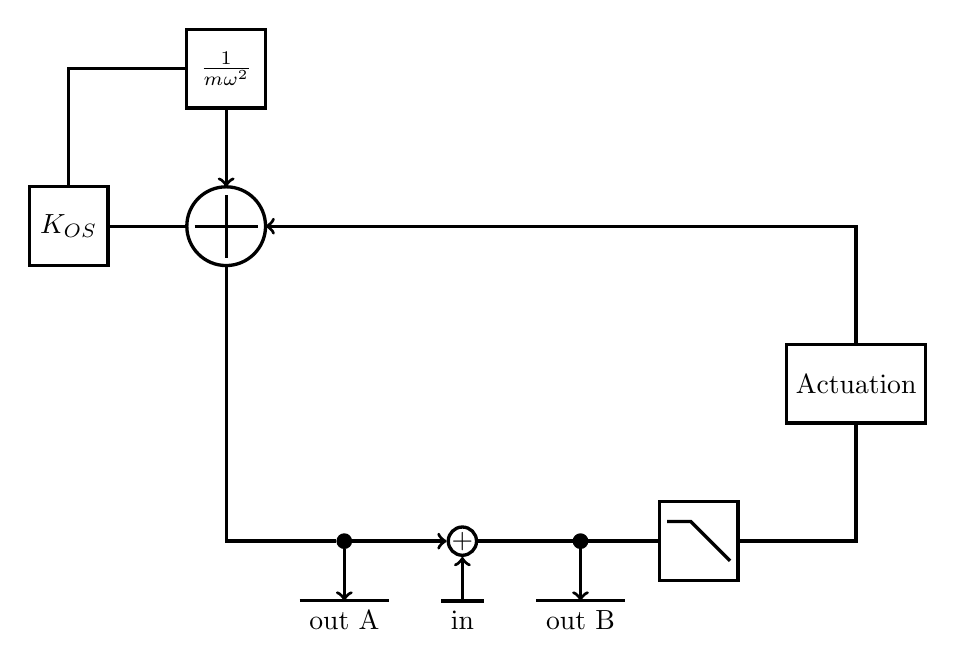
\begin{tikzpicture}
  [block/.style={rectangle,draw=black,very thick,align=center,
                  outer sep=0,minimum size=1cm,align=left},
   oscillator/.style={circle,draw=black,very thick,align=center,
                  outer sep=0,minimum size=1cm},
   digital/.style={rectangle,draw=black!50,fill=black!20,thick,align=center,
                   outer sep=0,minimum size=1cm,text width=0.9cm},
   physical/.style={rectangle,draw=green!50,fill=green!20,thick,align=center,
                    outer sep=0,minimum size=1cm,text width=0.9cm},
   spring/.style={rectangle,draw=red!50,fill=red!20,thick,align=center,
                   outer sep=0,minimum size=1cm,text width=0.9cm}]
  \node[circle,inner sep=0,draw,very thick] (sum) at (0,0) {+};
  \node[oscillator] (sumOS) at (-3,4) {};
  \draw[very thick] (-3.4,4) -- (-2.6,4);
  \draw[very thick] (-3,3.6) -- (-3,4.4);
  \node[block] (optspr) at (-5,4) {$K_{OS}$};
  \node[block] (mass) at (-3,6) {$\frac{1}{m\omega^2}$};
  \node[circle,outer sep=0,inner sep=0,fill=black,minimum size=0.2cm] (outa) at (-1.5,0) {};
  \node[circle,outer sep=0,inner sep=0,fill=black,minimum size=0.2cm] (outb) at (1.5,0) {};
  \node (outat) at (-1.5,-1) {out A};
  \node (outbt) at (1.5,-1) {out B};
  \node (int) at (0,-1) {in};
  \node[block] (filt1) at (3,0) {};
  \node[block] (actuation) at (5,2) {Actuation};
  \draw[very thick] (2.6,0.25) -- (2.9,0.25) -- (3.4,-0.25);
%  \node[oscillator] (mixer1) at (-3,0) {};
%  \draw[very thick] (-3,0) -- ++(45:0.5);
%  \draw[very thick] (-3,0) -- ++(135:0.5);
%  \draw[very thick] (-3,0) -- ++(225:0.5);
%  \draw[very thick] (-3,0) -- ++(315:0.5);
  \draw[very thick,->] (outa) -- (sum);
  \draw[very thick] (sum) -- (outb);
  \draw[very thick,->] (outa) -- (outat);
  \draw[very thick,->] (outb) -- (outbt);
  \draw[very thick,->] (int) -- (sum);
  \draw[very thick] (sumOS) |- (outa);
  \draw[very thick] (outb) -- (filt1);
  \draw[very thick] (filt1) -| (actuation);
  \draw[very thick,->] (actuation) |- (sumOS);
  \draw[very thick] (sumOS) -- (optspr);
  \draw[very thick] (optspr) |- (mass);
  \draw[very thick,->] (mass) -- (sumOS);
  \draw[very thick] (outat.north west) -- (outat.north east);
  \draw[very thick] (outbt.north west) -- (outbt.north east);
  \draw[very thick] (int.north west) -- (int.north east);
\end{tikzpicture}
\caption[Open Loop Gain Measurement]{This is a simplified schematic showing how
  we measure the optical spring.
  While the loop is closed, we can inject a sine wave of a specific frequency
  at "in", then measure the amplitude and phase shift of this sine wave at the
  points, outA and outB, giving us the complex numbers $A$ and $B$.
  The open loop gain at each point is then given by $A/B$
  The transfer function is then constructed out of many of these measurements
  at different frequencies.
  A Bode plot can then be made which is a plot of gain versus frequency.
  The plot is actually two plots: one for the magnitude of the gain and one
  for the phase of the gain.
  The transfer function we are measuring here is the open loop gain of the
  sensing, feedback, and actuation gain $H$ (the lower right loop) times the
  closed loop gain of the optical spring,
%  \begin{equation}
  $\mathrm{G} = \frac{H}{1-K_{OS}/m\omega^2}$.
%  \end{equation}
  }
\label{fig:results:servoloop}
\end{figure}

\section{Stability}

The definition of a stable system is one which has a bounded output for a
bounded input.
In our case we are interested in the closed-loop system consisting of an
optical spring attached to the small mass.
%if we apply a finite
%motion to the end of the spring opposite the mass, the motion of the mass must
%grow indefinitely.
%For us, our mass is a small mirror at one end of an optical
%spring cavity.

%The ideal system for us to work with is one that is linear and time-invariant
This system is linear and time-invariant
(LTI).
%This system can be well understood, and it is in the acheivement of a LTI
%system where much of our effort is focused.
%A system which is linear and time invariant
As such it will multiply a sinusoidal input
of a specific frequency with a complex number which is only dependant on this
frequency and will not change over time.
These values are called transfer function and fully describe the system.

The criterion for stability above translates into the requirement that all
poles of the transfer function lie in the upper half of the complex plane,
that is none of its eigenmodes are exponentially growing.
%Any signal (input) in the time domain can be expressed in a Fourier series, a sum
%of sinusoidal functions of different frequencies and amplitudes.
%The sinusoidal functions $e^{i\omega t}$ form a continuous basis set for the
%LTI system.
%As long as the output of a LTI system has $\Im(\omega) > 0$ the system is stable.
%But this definition is not directly useful for measuring stability.

%I will review the important points of the optical spring theory.
To convert this statement into a experimentally measurable criterion I first
look at the energy budget of the system.
As a reminder, a single optical spring has a delayed response in the cavity
which causes it to be unstable.
%The first thought is why? Why does that make it unstable?

One way to visualize this is that we have a system that, without the delay,
the force is maximum when the length is minimum.
%This is a critical point to be at because the energy that you put into the
%system is balanced, Work $=$ Force $\times$ Distance.
In this case as the cavity shortens, a force is applied in the opposite
direction.
As the cavity lengthens, a force is applied in the same direction as the motion.
And the total work done over each cycle is zero, $\oint F \mathrm{d}x = 0$.
With a positive delay, the force applied while the cavity is lengthening is
greater than when it is shortening which makes the total work per cycle greater
than zero.
We're adding energy to the system, making it unstable.
%This is only strictly valid at one instant in time because we are leaving out
%the effect that the force has on the motion of the mirror.

We can aid the visualization with the following thought experiment.
We attach a device that requires the mirror to follow a
sinusoidal motion at a specific amplitude and frequency regardless of external
forces and place it in a cavity to form an optical spring where the absolute
value of the spring constant is $m\omega_0^2$ where $m$ is the mass of the
optic\footnote{The imaginary device is massless of course.} and $\omega_0$
is the angular frequency the device is following.
Work would be done on the optic by the spring and taken up by the special device.
%In fact, assuming zero friction, the energy going into the device could be
%converted to lighting a bulb for instance.
Of course there's no magic here, the energy comes from the power delivered by
the laser.
Without the device to take up the energy the spring is delivering to
the optic, the energy must go into the motion of the optic where the total
energy is related to the motion by,
\begin{equation}
E = \frac{1}{2}kx_0^2 \;,
\end{equation}
where $k$ is the spring constant and $x_0$ is the amplitude of the motion.
A delay manifests itself in the transfer function as a phase lag.
To further work out how the transfer function phase is related to stability
we can solve the equations of motion,
\begin{align*}
F = ma &= -kx \\
  m\ddot x &= -kx\;.
\end{align*}
The solution to this is harmonic motion of the form,
\begin{align*}
x = Ae^{i\sqrt{k/m}t} + Be^{-i\sqrt{k/m}t} \;.
\end{align*}
I will take $B$ to be $0$. This sets the initial condition, which in the
end can be free again by multiplying by a phase factor $e^{i\theta}$.
Motion in the real world is real, so we always take the real part of the
complex motion when we're done. The imaginary part is just a mathematical
construct that helps with the calculations.

%Plots of the power from stable and unstable springs are shown in figure
%\ref{fig:otstabletime}.

We can damp the system in way similar to what was discussed in section
\ref{sec:II}. I will leave out the velocity term from equation
\ref{eqn:motion} and instead use a complex $k$ for the damping.
This is the same thing as having a viscosity coefficient $b$ with a $f^{-1}$
frequency dependence.
Allowing k to be a complex number, $k = k_0e^{i\phi}$,
we can see readily that this corresponds to a transfer function $-k$ which
shifts the wave in time.
%like we see in figure \ref{fig:otstabletime}.
%For  we can write $k=k_0e^{i\phi}$,
\begin{align}
F &= -kx \nonumber \\
  &= -k_0Ae^{i\omega t + i\phi} \;.
\end{align}
And the energy is,
\begin{align}
E &= \oint F\mathrm{d}x \nonumber \\
  &= \oint Fv\mathrm{d}t \nonumber \\
  &= \oint \Re\left( -k_0Ae^{i\omega t}e^{i\phi} \right)
    \Re\left( i\omega Ae^{i\omega t} \right) \mathrm{d}t \nonumber \\
  &= \frac{-k_0A^2}{2}\oint \Im\left(e^{i\phi}\right) \omega \mathrm{d}t \nonumber \\
  &= \frac{-k_0A^2}{2}\sin (\phi) \;.
\end{align}
We can see that with a
small positive $\phi$ we have a spring that is taking energy from the motion
of the mass. A small negative $\phi$ puts energy into the motion of the mass
making it unstable.
%If we were to have $A=0$ instead, the equivalent $k$ would be $k=k_0e^{-i\phi}$.
%In fact if we wanted to keep $A$ and $B$ the entire way, we could but it
%requires us to express the equations of motion with two dimensions,
%\begin{equation}
%\left( \begin{array}{cc} m & 0 \\ 0 & m \end{array} \right)
%  \left( \begin{array}{c} e^{i\omega t} \\ e^{-i\omega t} \end{array} \right)
%  = - \left( \begin{array}{cc} k_0e^{i\phi} & 0 \\ 0 & k_0e^{-i\phi} \end{array} \right)
%  \left( \begin{array}{c} e^{i\omega t} \\ e^{-i\omega t} \end{array} \right) \;.
%\end{equation}


%\begin{align}
%x &= Ae^{i\sqrt{k_0e^{i\phi}/m}t} \nonumber \\
%  &= Ae^{ie^{i\phi/2}\sqrt{k_0/m}t} \;.
%\end{align}
%Then, assuming $\phi$ is small, we'll set $\omega_0=\sqrt{k_0/m}$,
%\begin{align}
%x &= Ae^{i(1+i\phi/2)\omega_0t} + Be^{-i(1+i\phi/2)\omega_0t} \nonumber \\
%  &= Ae^{i\omega_0t}e^{\frac{-\phi}{2}\omega_0t} +
%    Be^{-i\omega_0t}e^{\frac{\phi}{2}\omega_0t} \nonumber \\
%  &= Ae^{i\omega_0t}e^{\frac{-\phi}{2}\omega_0t} +
%    Be^{-i\omega_0t}e^{\frac{\phi}{2}\omega_0t} \;.
%\end{align}

Looking at the transfer function of the closed loop and assuming $\phi \ll 1$,
\begin{align}
\mathrm{CLG} &= \frac{1}{1-\frac{k_0(1+i\phi)}{m\omega^2}} \nonumber \\
  &= \frac{m\omega^2}{m\omega^2-k_0(1+i\phi)} \;,
\end{align}
when the frequency is near resonance $m\omega^2 = k_0$,
the closed loop gain takes the form,
\begin{align}
&\frac{im\omega^2}{\phi} \nonumber \\
=&\frac{m\omega^2}{\phi}e^{i\pi/2} \;.
\end{align}
For a positive $\phi$, the phase of the transfer function goes through $\pi/2$
at the resonant frequency.
Conversely for the negative $\phi$, the phase goes through $-\pi/2$.
For the pure closed loop gain of a spring we see that the phase must be $-\pi$
below the resonant frequency and $0$ above the resonant frequency.
Therefore, for the case of the stable spring $\phi>0$, we see that the phase of
the transfer must decrease as the frequency increases through the resonance.
For the unstable spring $\phi<0$ the phase will increase over the resonance.
This can be seen in figure \ref{fig:dampedspringtf} and is experimentally
accessible in a closed loop measurement of the spring.

Now, in our case, the measurement isn't the pure closed loop gain of the
optical spring.
We are actually measuring this closed loop gain times the open loop gain of the
feedback loop.
The result is that the characteristic shape of the falling phase over the
resonance preserved.
This can be seen by writing the complex gains with exponential functions to
generate the imaginary parts,
\begin{align}
FG &= F_0e^{i\theta_1}G_0e^{i\theta_2} \nonumber \\
  &= F_0G_0e^{i(\theta_1+\theta_2)} \;,
\end{align}
where $G$ is the closed loop transfer function for the optical spring and
$F$ is the transfer function for the rest of the feedback system.
Knowing $\theta_1$ we can subtract it from the measured phase.
I will actually present the results as they were measured and compare with the
theoretical plot of the transfer function including both the optical spring
closed loop transfer function and the feedback transfer function.

\subsection{Stability Range}
\label{sec:results_stability}
We know how to make a stable spring but any spring becomes nonlinear at some
range of motion.
For us to be able to remove the active feedback to the system, we
need to understand what this range is so we can stay within its limits.
We can first define a region of stability where the phase of the spring is
positive.
An example parameter space is shown in figure \ref{fig:experiment2space}.
On the y-axis of this plot you see the subcarrier detuning. This is the
overall detuning of the cavity in frequency, which directly corresponds to
a cavity length by,
\begin{equation}
\frac{\Delta L}{L} = \frac{\Delta f}{f} \label{eq:lengthtofreq} \;,
\end{equation}
Where $L$ is the length of the cavity and $f$ is the frequency of the laser.
The x-axis changes the nature of the double optical field that we're sending
into the cavity.
It is completely indepedent of the cavity length change.

We want the mirror to stay within the limits of positive phase, which is within
the zero phase line on the plot.
If we pick a spot along the x-axis and vary the subcarrier offset
(or mirror position) we see that the frequency of the spring increases quite a
bit from the center of the stable range.
Additionally, the phase of the spring decreases to zero.
To give a margin, we will want the range of motion to really stay within about
a tenth of the overall stable boundary.
Looking at the blue star in this plot, we can see that the frequency and phase
of the spring don't change dramatically within about 10kHz of subcarrier
detuning compared to the $\approx 100$ kHz stable region. By equation
\eqref{eq:lengthtofreq} we get a length displacement of,
\begin{align}
\Delta L &= \frac{10\mathrm{kHz}}{2.8\times 10^{11}\mathrm{kHz}}
    0.07\mathrm{m} \nonumber \\
  &= 2.5 \mathrm{pm} \;.
\end{align}

Because the spring frequency actually increases toward the boundary, more force
is required to get the spring into the unstable region than what one would
compute from the central k value with $F=-kx$.
We would actually need a force of $m\omega^2 x$ to get into the region of
instability, where $\omega$ is the spring angular frequency at the boundary.
For example, in the case of the blue star from the plot, the lower spring
frequency at the boundary is $f_\mathrm{limit} = 800\mathrm{Hz}$.
The force required to exceed this boundary will be then given by,
\begin{align*}
F &= 4\pi^2mf_\mathrm{limit}^2x \\
  &= 4\pi^2 \times 0.0005 \mathrm{kg} \times (800\mathrm{Hz})^2 \times 10
     \mathrm{pm} \\
  &= 1.26 \times 10^{-7} \mathrm{N} \;.
\end{align*}
This is all good for the adiabatic case where the motion is less than the spring
resonance.
The resonantly enhanced motion at the spring resonance, however, is strongly
dependant on the phase of the spring.
The damped spring removes energy entering the system at a rate determined by
the phase.
Since we are not always at the equilibrium point, the average phase and
therefore the average amount of energy dissipated is less than at the
equilibrium point, effectively increasing the $Q$ of the spring.

Since we have a high $Q$ optical spring most of the \ac{rms} motion of the mass
will come from the amplification at the resonance until we include very low
frequency motion.
As we go lower in frequency the optical spring filters out more of the motion
as seen in figure \ref{fig:dampedspringtf}.
This decreases as $f^2$ until we get to the suspension resonance, which is not
shown in the plot.
At frequencies below this point, the optical spring response flattens out
and no longer depends on the frequency.
Our suspension resonance is at about 18Hz and below this point, the amount
of displacement noise due to seismic starts to become the dominant noise
source.
At low enough frequencies, if the optical spring is not strong enough, the
seismic motion will dominate the total \ac{rms} motion.
The closed loop suppression at frequencies below the suspension resonance can
be found easily since we know the transfer function is 1 at very high
frequencies and $f^2$ between the the suspension resonance and the optical
resonance.
The suspression below the suspension frequency is then,
\begin{align}
\left( f_\mathrm{sus}/f_\mathrm{OS} \right)^2 \;,
\end{align}
which with an optical spring frequency of 720 Hz we have seismic supression of,
\begin{align*}
& \left(\frac{1}{40}\right)^2 \\
&= \frac{1}{1600} \\
&\approx 6\times 10^{-4} \;.
\end{align*}
At very low frequencies, where the \ac{rms} motion will increase again, we are
in the adiabatic condition and have the advantage of the steep energy
boundaries of the spring. An example of two different spring configurations can
be seen in figure \ref{fig:rmsspringcompare}.

\begin{figure}
  \centering
  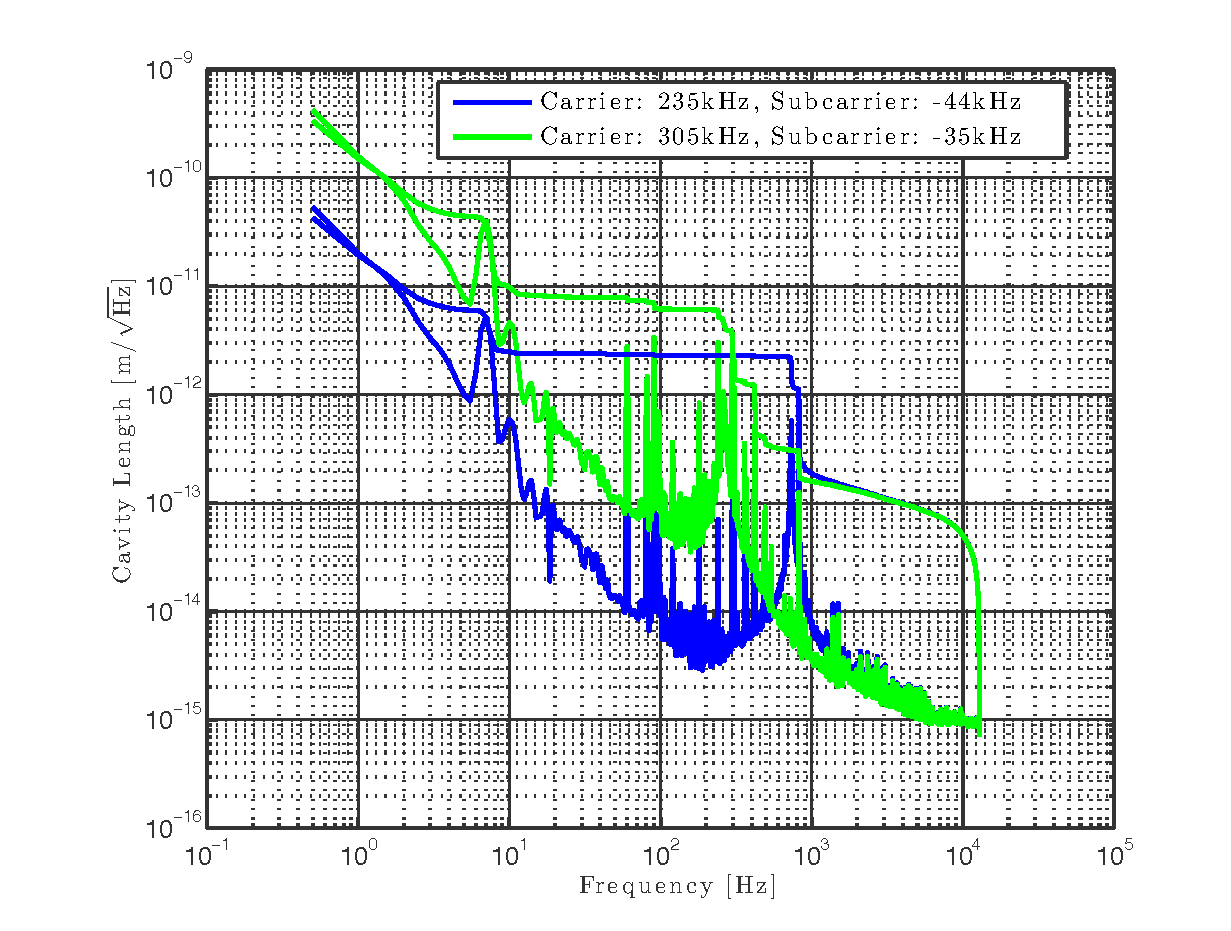
\includegraphics[width=14cm]{./figures/rmsspringcompare.pdf}
  \caption[RMS Optical Spring Residual Motion]{
    RMS motion after applying optical spring.
    The carrier and subcarrier input powers are fixed for both examples.
    The subcarrier detuning was chosen to maximize the damping for each
    carrier detuning.
    This plot uses the noise measurement from section 
    includes the coefficient of thermal expansion term that
    is discussed in section \ref{sec:opticthermalexpansion}.
    }
  \label{fig:rmsspringcompare}
\end{figure}





\begin{figure}
  \centering
  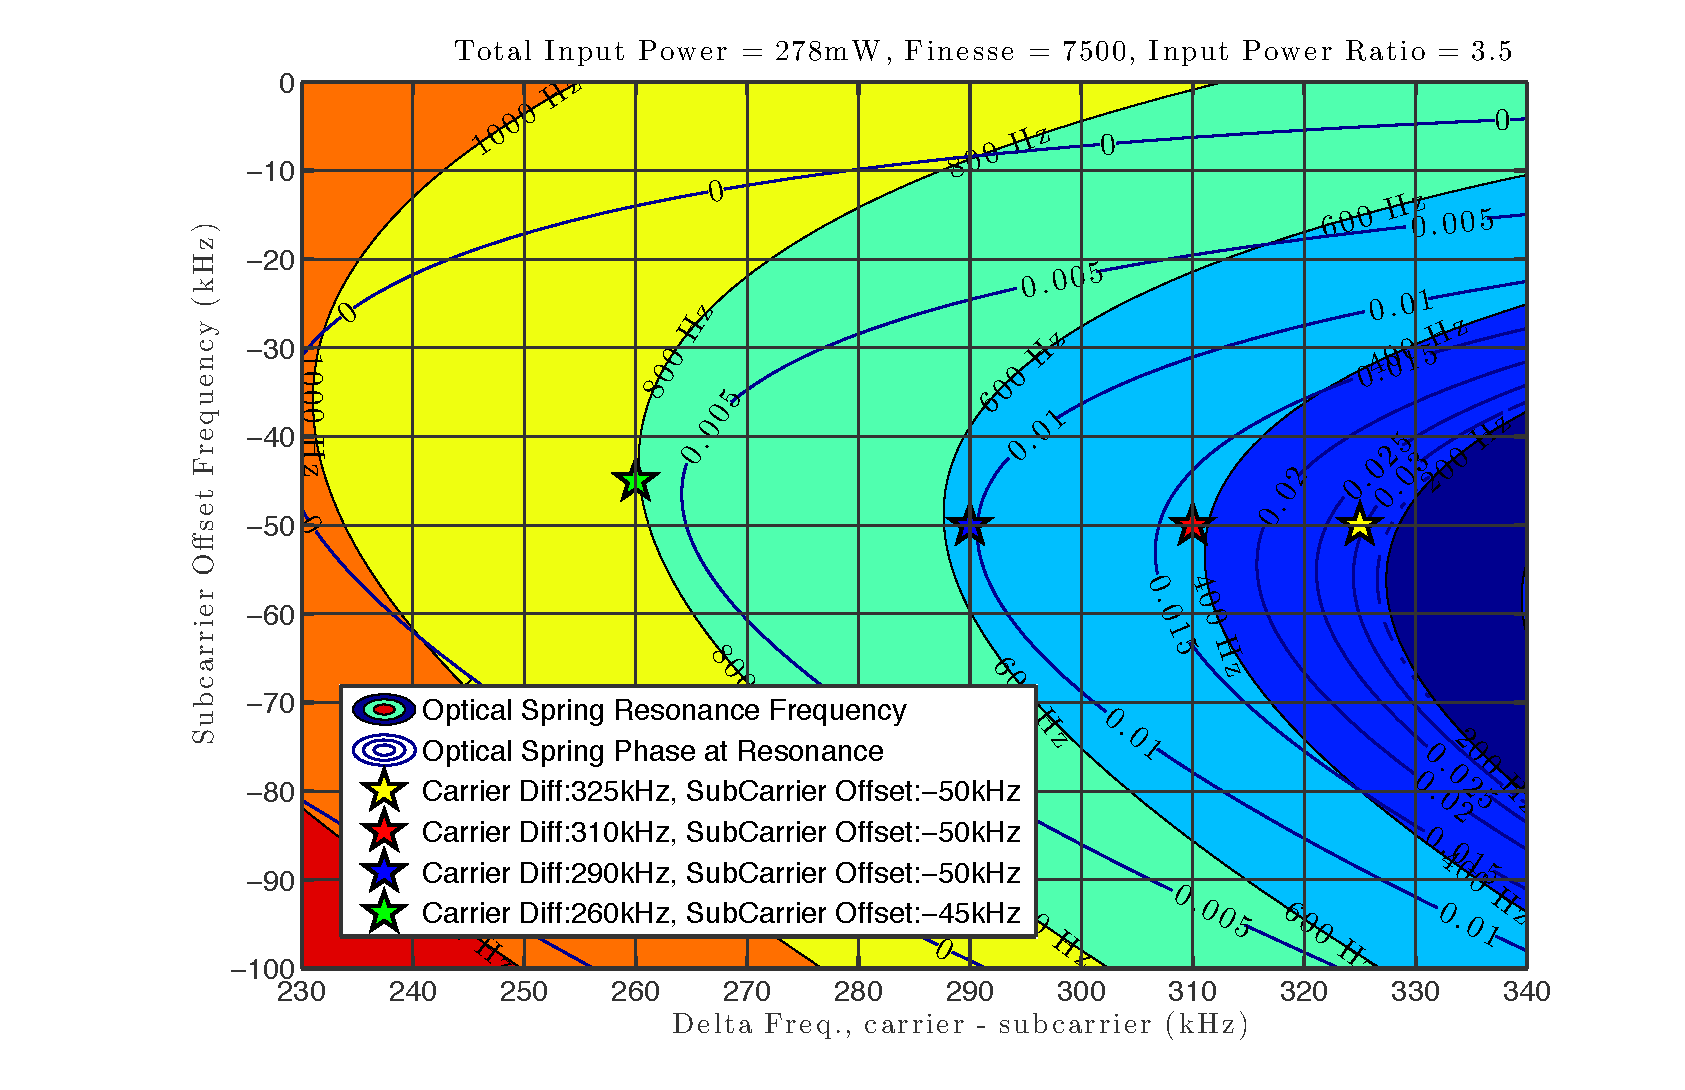
\includegraphics[width=14cm]{./figures/experiment2space.pdf}
  \caption[Parameter Space for 2nd Edition]{The parameter space of the
    experiment.
    We can see the stability values for different detunings given
    by the phase contours which are in units of radians.
    Ideally we want a high frequency and phase.
    }
  \label{fig:experiment2space}
\end{figure}

%\begin{figure}
%\centering
%\tikzsetnextfilename{OT_stable_time}
%\begin{tikzpicture}
%  \begin{axis}[
%    name=plot1,
%    height=6cm,
%    ymax=2.5,
%    xlabel={$\mathrm{Time} [\mathrm{s}]$},
%    ylabel={$\mathrm{Amplitude [1]}$},
%    legend cell align=left,
%    legend style={font=\scriptsize},
%    grid=major,
%    ]
%  \addplot[very thick,samples=200,domain=-3:3,blue!80!black] {sin(x*360)};
%  \addlegendentry{$\sin (2\pi ft)$};
%  \addplot[very thick,samples=200,domain=-3:3,red!80!black] {-sin((x+0.1)*360)};
%  \addlegendentry{$-\sin (2\pi f(t + 0.1))$};
%  \addplot[very thick,samples=200,domain=-3:3,green!80!black] {-cos(x*360)*sin((x+0.1)*360)};
%  \addlegendentry{$-\cos(2\pi ft) \sin (2\pi f(t+0.1))$};
%  \end{axis}
%  \begin{axis}[
%    name=plot2,
%    at=(plot1.below south), anchor=above north,
%    height=6cm,
%    ymax=2.5,
%    xlabel={$\mathrm{Time} [\mathrm{s}]$},
%    ylabel={$\mathrm{Amplitude [1]}$},
%    legend cell align=left,
%    legend style={font=\scriptsize},
%    grid=major,
%    ]
%  \addplot[very thick,samples=200,domain=-3:3,blue!80!black] {sin(x*360)};
%  \addlegendentry{$\sin (2\pi ft)$};
%  \addplot[very thick,samples=200,domain=-3:3,red!80!black] {-sin((x-0.1)*360)};
%  \addlegendentry{$-\sin (2\pi f(t - 0.1))$};
%  \addplot[very thick,samples=200,domain=-3:3,green!80!black] {-cos(x*360)*sin((x-0.1)*360)};
%  \addlegendentry{$-\cos(2\pi ft) \sin (2\pi f(t-0.1))$};
%  \end{axis}
%\end{tikzpicture}
%\caption[Damped Spring Energy Flow]{This shows the power being delivered to a mass
%  attached to a spring where a device keeps the motion of the mass at a fixed
%  frequency and amplitude as given by the blue trace.
%  This device is simply provided as a tool for this thought experiment and is
%  not an actual device we use in the lab experiment.
%  The spring applies a force (red trace) opposite to the displacement of the mass
%  from equilibrium but with a time shift.
%  The green trace is the power delivered to the mass by the spring.
%  From the upper plot you can see that the spring is actually taking energy out
%  of the system.
%  In the lower plot the spring is providing energy to the system.
%  In both cases, since we have our special device to keep the motion constant,
%  the energy flows into and out of this device.
%  An ordinary spring does not provide a continuous energy source but it can take
%  energy out of the system in the form of friction.
%  Our optical spring on the other hand has a continuous energy source from the
%  laser itself.
%  The difference in power is applied to the total of the reflected and
%  transmitted beams from the cavity.
%  }
%\label{fig:otstabletime}
%\end{figure}

\begin{figure}
\centering
\tikzsetnextfilename{dampedTF}
\begin{tikzpicture}
  \begin{loglogaxis}[
    name=plot1,
    height=6cm,
%    xlabel={$\mathrm{Frequency} [\mathrm{Hz}]$},
    ylabel={$\mathrm{Magnitude}$},
    legend cell align=left,
    legend style={font=\scriptsize},
    grid=major,
    ]
    \addplot[blue,very thick] table[x index=0,y index=1]
      {./matlab_traces/damposcmag.dat};
    \addlegendentry{$\phi = +0.05$};
    \addplot[red,very thick] table[x index=0,y index=2]
      {./matlab_traces/damposcmag.dat};
    \addlegendentry{$\phi = +0.1$};
    \addplot[green,dashed,very thick] table[x index=0,y index=3]
      {./matlab_traces/damposcmag.dat};
    \addlegendentry{$\phi = -0.05$};
    \addplot[yellow,dashed,very thick] table[x index=0,y index=4]
      {./matlab_traces/damposcmag.dat};
    \addlegendentry{$\phi = -0.1$};
  \end{loglogaxis}
  \begin{semilogxaxis}[
    name=plot2,
    at=(plot1.below south), anchor=above north,
    height=6cm,
    xlabel={$\mathrm{Frequency} [\mathrm{Hz}]$},
    ylabel={$\mathrm{Phase [Deg]}$},
    legend cell align=left,
    legend style={font=\scriptsize},
    grid=major,
    ]
    \addplot[blue!80!black,very thick] table[x index=0,y index=1]
      {./matlab_traces/damposcphase.dat};
    \addplot[red!80!black,very thick] table[x index=0,y index=2]
      {./matlab_traces/damposcphase.dat};
    \addplot[green!80!black,dashed,very thick] table[x index=0,y index=3]
      {./matlab_traces/damposcphase.dat};
    \addplot[yellow!80!black,dashed,very thick] table[x index=0,y index=4]
      {./matlab_traces/damposcphase.dat};
%    \addplot[very thick,smooth,samples=2000,domain=1:100,blue!80!black]
%      {atan(100*0.05/(x^2-100))};
%      {1/sqrt((1-100/x^2)^2+(100/x^2*0.05)^2)};
%    \addlegendentry{OLG};
%    \addplot[very thick,smooth,samples=2000,domain=1:100,red!80!black]
%      {atan(100*0.1/(x^2-100))};
%      {1/sqrt((1-100/x^2)^2+(100/x^2*0.1)^2)};
%    \addlegendentry{OLG};
  \end{semilogxaxis}
\end{tikzpicture}
\caption[Damped Spring Closed Loop Gain]{
  Damped spring closed loop gain behavior.
  The two solid lines are examples of stable springs ($\phi>0$).
  The two dashed lines are unstable springs.
  The signature we look for to verify stability of the optical spring is
  the direction the phase goes from 180 to 0 degrees.
  Decreasing phase over the resonant frequency indicates a stable spring, while
  the unstable spring has the opposite behavior.
  Notice that the stability cannot be determined from the magnitude plot.
  Positive and negative $\phi$ look exactly the same.
  Loss angle $\phi$ is presented in radians.
  }
\label{fig:dampedspringtf}
\end{figure}



%\section{Measurements}
%
%Linear trap measurements have been taken twice.
%The first measurement was with the subcarrier at the same offset frequency from
%the carrier for each measurement.
%The results generally were in line with the theory, however there were
%complications from the layout which needed to be addressed.

\section{Linear Trap Experiment, 1st Edition}

%\begin{figure}[htbp]
%    \centering
%    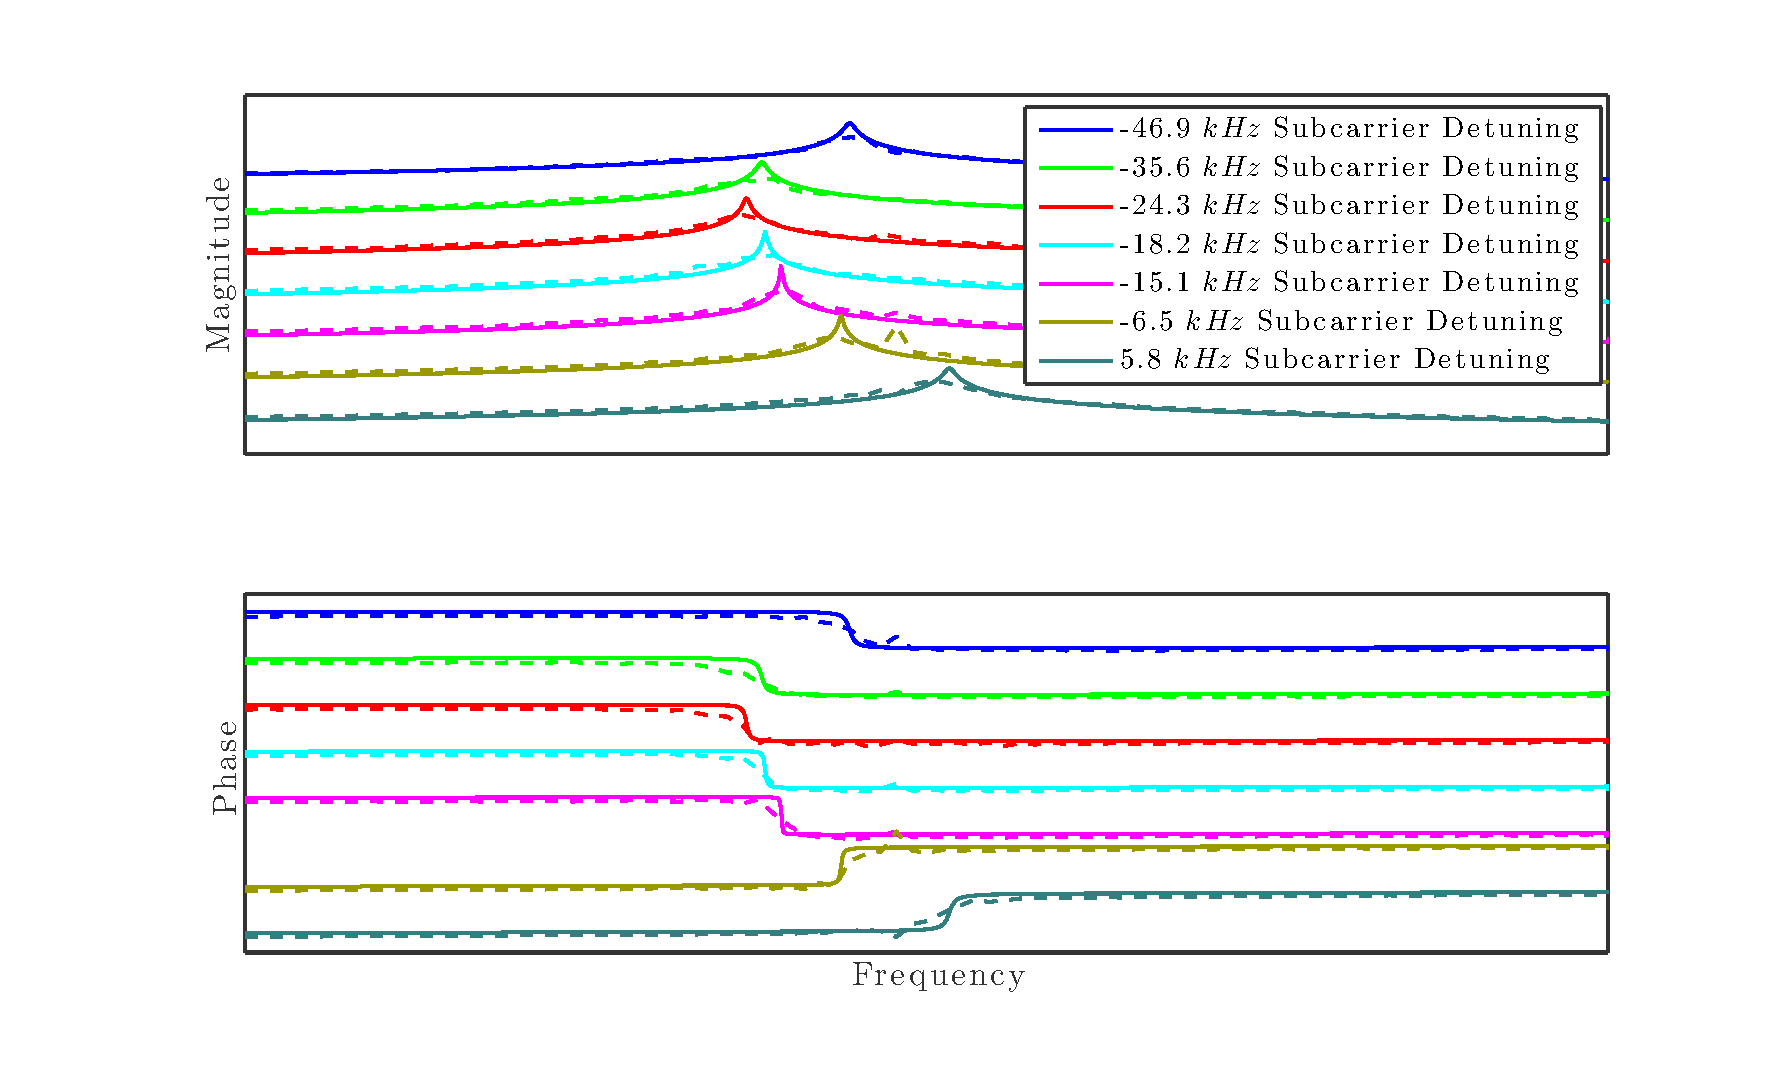
\includegraphics[width=20cm]{./figures/april_results_olgfit.eps}
%    \caption[Data Fitting of Open Loop Gain for 1st Results]{This is the open
%        loop gain fit of the last 7 measurements taken during a segment of
%        time in which the cavity was continuously locked.
%        The trap cavity had been locked for a few hours at this point and
%        seemed to have stabilized compared to earlier in the lock segment.
%        These measurements were taken no more than 5 minutes apart from each
%        other so the effects of any drifted were minimized.}
%    \label{fig:olgapril}
%\end{figure}

In the first set of measurements, the carrier to subcarrier power ratio was
set to 10.
I fixed the subcarrier to carrier offset frequency to 355kHz.
This offset frequency was chosen because it gave a comfortable margin
in stability.
The trap would consistently lose lock with an offset of around
250kHz.
A list of parameters is provided in table \ref{tab:trapparams1}.

\begin{table}
  \begin{center}
    \begin{tabular}{|l|l|l|}
      \hline
      Parameter & Value & Units \\
      \hline
      \hline
      Cavity Length & 7 & cm \\
      Carrier Power & 440 & mW \\
      Subcarrier Power & 44 & mW \\
      Subcarrier Servo Offset & 355 & kHz \\
      PDH Local Oscillator & 35 & MHz \\
      Specified EOM Modulation Depth & $>0.2$ & rad/V \\
%      Local Oscillator Power (EOM) & & \\
      \hline
    \end{tabular}
  \end{center}
  \caption[Parameters for Linear Trap Experiment, 1st Edition]{
      Parameters for the first edition of the linear trap experiment.
      }
  \label{tab:trapparams1}
\end{table}


The experiment was performed by keeping the power constant for each beam,
leaving the carrier frequency offset by 355kHz above the subcarrier frequency,
and varying the subcarrier detuning.
With this, when the subcarrier is detuned above the resonant frequency of the
cavity, both beams are detuned in the same direction and the resulting
combined spring must be unstable.
We expect that as we detune the subcarrier from positive to negative the
contribution to the spring constant from the subcarrier will decrease which
in turn reduces the resonant frequency.
Because of the power ratio, cavity finesse, and subcarrier servo offset
frequency we expect to see stable springs at some point after detuning the
subcarrier beam to the opposite side of the resonant frequency of the cavity.
%This is illustrated in figure \ref{fig:paramspace1}.

During the optical spring measurements we were sensitive to variations in
power.
I observed that the stable optical spring frequency could drift over a few
hours by as much as 100Hz without me changing any of the parameters of the
setup.
%This is shown in figure \ref{fig:stablefixedoffset}.
This is shown in table \ref{tab:experiment1lock2}.

\begin{table}
  \begin{center}
    \footnotesize
    \begin{tabular}{|l|l|l|l|}
      \hline
      Measurement ID & Error point offset $[\mathrm{mV}]$ &
        Resonant Frequency [Hz] & Time of Measurement [Min] \\
      \hline
      \hline
      1-30 & -604  & 742 & 0 \\
      1-31 & -873  & 757 & 4 \\
      1-33 & -1120 & 782 & 9 \\
      1-34 & -1410 & 834 & 12 \\
      1-35 & -827  & 768 & 17 \\
      1-36 & -827  & 789 & 52 \\
      1-37 & -827  & 870 & 91 \\
      1-38 & -827  & 820 & 102 \\
      1-39 & -522  & 800 & 107 \\
      1-40 & -172  & 797 & 112 \\
      1-41 & 28    & 801 & 117 \\
      1-42 & 137   & 806 & 120 \\
      1-43 & 438   & 818 & 125 \\
      1-44 & 879   & 840 & 130 \\
      \hline
    \end{tabular}
  \end{center}
  \caption[Experiment 1 Spring Measurements]{
      This table contains the error point offset measured for each spring
      measurement during the second lock stretch of experiment 1.
      The frequencies indicated were measured from the data by finding the
      frequency corresponding to the $\pm 90$ degree phase point of the closed
      loop optical spring.
      Measurements 35-38 were taken at the same error point offset and had
      a wide range in resonant frequencies compared to the rest of the data.
      Measurement ID 1-32 is not included in this table because the data was
      saved twice.
      The data is identical to 1-33.
      }
  \label{tab:experiment1lock2}
\end{table}

%\begin{figure}
%\centering
%\tikzsetnextfilename{stablefixedoffset}
%\begin{tikzpicture}
%  \small
%  \begin{loglogaxis}[
%    name=plot1,
%    height=5cm,
%    xmin=400,
%    xmax=2000,
%    xtick={400,500,600,700,800,900,1000,2000},
%%    log basis x=10,
%    log ticks with fixed point,
%%    xlabel={$\mathrm{Frequency} [\mathrm{Hz}]$},
%    ylabel={$\mathrm{Magnitude}$},
%    legend cell align=left,
%    legend style={font=\scriptsize},
%    grid=both,
%    ]
%    \addplot[blue,very thick] table[x index=0,y index=1]
%      {./matlab_traces/april_olg_35.dat};
%    \addplot[red,very thick] table[x index=0,y index=1]
%      {./matlab_traces/april_olg_36.dat};
%    \addplot[green,very thick] table[x index=0,y index=1]
%      {./matlab_traces/april_olg_37.dat};
%    \addplot[orange,very thick] table[x index=0,y index=1]
%      {./matlab_traces/april_olg_38.dat};
%  \end{loglogaxis}
%  \begin{semilogxaxis}[
%    name=plot2,
%    at=(plot1.below south), anchor=above north,
%    height=5cm,
%    xmin=400,
%    xmax=2000,
%    xtick={400,500,600,700,800,900,1000,2000},
%%    log basis x=10,
%    log ticks with fixed point,
%    xlabel={$\mathrm{Frequency} [\mathrm{Hz}]$},
%    ylabel={$\mathrm{Phase}$},
%    legend cell align=left,
%    legend style={font=\scriptsize},
%    grid=both,
%    ]
%    \addplot[blue,very thick] table[x index=0,y index=2]
%      {./matlab_traces/april_olg_35.dat};
%    \addplot[red,very thick] table[x index=0,y index=2]
%      {./matlab_traces/april_olg_36.dat};
%    \addplot[green,very thick] table[x index=0,y index=2]
%      {./matlab_traces/april_olg_37.dat};
%    \addplot[orange,very thick] table[x index=0,y index=2]
%      {./matlab_traces/april_olg_38.dat};
%  \end{semilogxaxis}
%\end{tikzpicture}
%\caption[]{}
%\label{fig:stablefixedoffset}
%\end{figure}

After the data was taken of the stable spring with fixed parameters and before
losing lock on the feedback loop, I took several measurements in a row in a
shorter period of time of about 30 minutes total. The results from these
measurements are provided in figures \ref{fig:april_space1}, and
\ref{fig:aprilolg1}.

One of the reasons for this is the fact that the carrier beam was not
well aligned to the subcarrier beam causing drifts in the power ratio between
carrier and subcarrier as the overall alignment drifted.
Another complication in the first run was due to the fact that the carrier and
subcarrier beams had exactly the same polarizations which caused a strong
beat signal at 355kHz. This beat signal was low enough in frequency that
it would show strongly in the resonant \ac{rfpd} output, likely causing
saturation effects in the electronics that would lead to an unpredictable
subcarrier detuning.
The effect of carrier and subcarrier beating will be discussed further in
section \ref{sec:expimps}

Changing the detuning of the subcarrier during the measurement also changes the
overall gain of the feedback system.
This is because of the fact that the \ac{pdh} error signal does not have a
linear relationship with detuning as seen in figure \ref{fig:pdh}.
During each measurement, we keep the error point fixed to a small region,
which keeps the system quite linear.
But as we change the error point offset the slope of the signal changes.
This slope corresponds to an overall gain factor in the system.
We can actually see the effect in the measurements of figure
\ref{fig:aprilolg2}.


Despite these issues we were clearly able to observe
stable and unstable optical springs and there was a short stretch of
measurements that were able to be fit to the theoretical model.
However, to get the actual frequency detuning and power level under better
control, a few design changes were needed which I will discuss in the next
section.


\begin{figure}
  \tikzsetnextfilename{april_space1}
  \begin{tikzpicture}
  \begin{axis}[
    name=plot1,
    height=8cm,
    width=14cm,
    ylabel={Resonant Frequency $\left[\mathrm{Hz}\right]$ },
    xlabel={Subcarrier Detuning $\left[\mathrm{kHz}\right]$},
    grid=major,
  ]
  \addplot[blue,very thick] table[x index=1,y index=2]
    {./matlab_traces/april_fitspace_stable.dat};
  \addplot[green,very thick] table[x index=1,y index=2]
    {./matlab_traces/april_fitspace_unstable.dat};
  \addplot[blue,only marks] table[x index=1,y index=2]
    {./matlab_traces/april_pointspace_stable.dat};
  \addplot[green,only marks] table[x index=1,y index=2]
    {./matlab_traces/april_pointspace_unstable.dat};
  \end{axis}
  \end{tikzpicture}
    \caption[Parameters from the 1st Edition]{
      The solid lines show the theoretical
      spring frequencies for all of the measurements that took place in a span
      of about 30 minutes during the first edition at the end of one lock
      stretch.
      The dots correspond to the actual measurements of the optical spring at
      different subcarrier detunings. The entire space depicted is in the region
      of static stability, i.e. the optical spring provides a restoring force.
      The colors correspond to the dynamic stability of the optical spring.
      Blue is dynamically stable.
      Green is dynamically unstable.
      The carrier frequency remained at a fixed offset from the subcarrier at
      355 kHz.
      The fitting for this plot was done by plotting the actual measured
      resonant frequency vs. the error point offset in mV.
      The theoretical curve was transformed to match the axes using the
      \ac{pdh} transformation shown in figure \ref{fig:pdh}.
      I could then fit the curve using four parameters:
      finesse, total power, error point voltage offset,
      and carrier to subcarrier power ratio.
      The parameters used in this plot are:
      $\mathcal{F}=8000$, power ratio$=1.5$, total power$=344.7\mathrm{mW}$,
      error point offset$=-670\mathrm{mV}=-19.07\mathrm{kHz}$.
      This does not include any effect due to the thermal expansion of the
      optics mentioned in section \ref{sec:opticthermalexpansion}.
      }
  \label{fig:april_space1}
\end{figure}

\begin{figure}
  \tikzsetnextfilename{april_olg1}
  \begin{tikzpicture}
  \begin{semilogyaxis}[
    name=plot1,
    height=5cm,
    width=7cm,
    xmin=760,
    xmax=880,
    ylabel={Magnitude},
    grid=major,
  ]
  \addplot[blue,very thick] table[x index=0,y index=1] {./matlab_traces/april_olg_38.dat};
  \addplot[blue] table[x index=0,y index=1] {./matlab_traces/april_fit.dat};
  \addplot[red,very thick] table[x index=0,y index=1] {./matlab_traces/april_olg_39.dat};
  \addplot[red] table[x index=0,y index=3] {./matlab_traces/april_fit.dat};
  \addplot[green,very thick] table[x index=0,y index=1] {./matlab_traces/april_olg_40.dat};
  \addplot[green] table[x index=0,y index=5] {./matlab_traces/april_fit.dat};
  \end{semilogyaxis}


  \begin{axis}[
    name=plot3,
    at=(plot1.below south), anchor=north,
    height=5cm,
    width=7cm,
    xmin=760,
    xmax=880,
    xlabel={Frequency $\left[\mathrm{Hz}\right]$},
    ylabel={Phase},
    grid=major,
  ]
  \addplot[blue,very thick] table[x index=0,y index=2] {./matlab_traces/april_olg_38.dat};
  \addplot[blue] table[x index=0,y index=2] {./matlab_traces/april_fit.dat};
  \addplot[red,very thick] table[x index=0,y index=2] {./matlab_traces/april_olg_39.dat};
  \addplot[red] table[x index=0,y index=4] {./matlab_traces/april_fit.dat};
  \addplot[green,very thick] table[x index=0,y index=2] {./matlab_traces/april_olg_40.dat};
  \addplot[green] table[x index=0,y index=6] {./matlab_traces/april_fit.dat};
  \end{axis}
  \begin{axis}[
    name=plot4,
    at=(plot3.east), anchor=left of west,
    height=5cm,
    width=7cm,
    xmin=760,
    xmax=880,
    xlabel={Frequency $\left[\mathrm{Hz}\right]$},
    ylabel={Phase},
    grid=major,
  ]
  \addplot[blue,very thick] table[x index=0,y index=2] {./matlab_traces/april_olg_41.dat};
  \addplot[blue] table[x index=0,y index=8] {./matlab_traces/april_fit.dat};
  \addplot[red,very thick] table[x index=0,y index=2] {./matlab_traces/april_olg_42.dat};
  \addplot[red] table[x index=0,y index=10] {./matlab_traces/april_fit.dat};
  \addplot[green,very thick] table[x index=0,y index=2] {./matlab_traces/april_olg_43.dat};
  \addplot[green] table[x index=0,y index=12] {./matlab_traces/april_fit.dat};
  \addplot[black,very thick] table[x index=0,y index=2] {./matlab_traces/april_olg_44.dat};
  \addplot[black] table[x index=0,y index=14] {./matlab_traces/april_fit.dat};
  \end{axis}

  \begin{semilogyaxis}[
    name=plot2,
    at=(plot4.north), anchor=below south,
    height=5cm,
    width=7cm,
    xmin=760,
    xmax=880,
    ylabel={Magnitude},
    grid=major,
  ]
  \addplot[blue,very thick] table[x index=0,y index=1] {./matlab_traces/april_olg_41.dat};
  \addplot[blue] table[x index=0,y index=7] {./matlab_traces/april_fit.dat};
  \addplot[red,very thick] table[x index=0,y index=1] {./matlab_traces/april_olg_42.dat};
  \addplot[red] table[x index=0,y index=9] {./matlab_traces/april_fit.dat};
  \addplot[green,very thick] table[x index=0,y index=1] {./matlab_traces/april_olg_43.dat};
  \addplot[green] table[x index=0,y index=11] {./matlab_traces/april_fit.dat};
  \addplot[black,very thick] table[x index=0,y index=1] {./matlab_traces/april_olg_44.dat};
  \addplot[black] table[x index=0,y index=13] {./matlab_traces/april_fit.dat};
  \end{semilogyaxis}

  \end{tikzpicture}
    \caption[Data Fitting of Open Loop Gain for 1st Results]{This is the open
        loop gain fit of the last 7 measurements taken during a segment of
        time in which the cavity was continuously locked.
        The three traces in the top two plots are of the stable spring with
        a large negative detuning.
        They correspond to the three blue dots from figure
        \ref{fig:april_space1} with the most negative subcarrier detuning.
        The thick traces in all plots are from the measurements in the lab.
        The thin traces are of the modelled open loop gain.
        The trap cavity had been locked for a few hours at this point and
        seemed to have stabilized compared to earlier in the lock segment.
        These measurements were taken no more than 5 minutes apart from each
        other so the effects of any drifting were minimized.}
  \label{fig:aprilolg1}
\end{figure}

\begin{figure}
  \centering
  \tikzsetnextfilename{aprilolg2}
  \begin{tikzpicture}
    \begin{axis}[
      ylabel={Magnitude},
      xlabel={Frequency[Hz]},
      height=6cm,
%      xmin=1500,
%      xmax=2000,
%      ymin=5,
%      ymax=20,
      legend style={legend pos=north east,font=\small},
      grid=both,
      ]
      \addplot[blue,very thick] table[x index=0,y index=1]
        {./matlab_traces/april_olg_zoom_38.dat};
      \addlegendentry{-872 mV};
      \addplot[red,very thick] table[x index=0,y index=1]
        {./matlab_traces/april_olg_zoom_39.dat};
      \addlegendentry{-522 mV};
      \addplot[green,very thick] table[x index=0,y index=1]
        {./matlab_traces/april_olg_zoom_40.dat};
      \addlegendentry{-172 mV};
      \addplot[brown,very thick] table[x index=0,y index=1]
        {./matlab_traces/april_olg_zoom_41.dat};
      \addlegendentry{28 mV};
      \addplot[yellow,very thick] table[x index=0,y index=1]
        {./matlab_traces/april_olg_zoom_42.dat};
      \addlegendentry{137 mV};
      \addplot[orange,very thick] table[x index=0,y index=1]
        {./matlab_traces/april_olg_zoom_43.dat};
      \addlegendentry{438 mV};
      \addplot[magenta,very thick] table[x index=0,y index=1]
        {./matlab_traces/april_olg_zoom_44.dat};
      \addlegendentry{879 mV};
    \end{axis}
  \end{tikzpicture}
  \caption[Subcarrier Detuning Gain Factor]{
    Relative gain above resonant frequency for different subcarrier detunings.
    The peak gain appears to be at an offset of about 250mV which contradicts
    the fit in figure \ref{fig:april_space1}.
    This provides further motivation to constrain the measurements better
    by monitoring key parameter needed to fit the model.
    }
  \label{fig:aprilolg2}
\end{figure}

\section{Experimental Layout Revision}
\label{sec:expimps}
From our first layout design there was a rather
large beat signal on the \ac{rfpd} used for generating the \ac{pdh} signal
for our locking feedback servo.
This beat signal is a result of our initial layout involving the combining of
carrier and subcarrier beams before a \ac{fi} which resulted in the two beams
having the same polarization.
This produces a beat signal of the difference in the two frequencies.
The power inside the cavity has the beat between the carrier beam
and the unmodulated part of the subcarrier beam. This shows up in the
transmitted DC \ac{pd} because the bandwidth is much greater than the
subcarrier servo offset frequency. The Thorlabs PD10CS set to 0dB gain has
a bandwidth of 17MHz.
In the resonant \ac{rfpd} we see the beat between the carrier beam and the
sideband of the subcarrier beam because the linewidth of the resonance
in the \ac{pd} is also greater than the subcarrier servo offset frequency.
For a subcarrier offset of 355kHz, the \ac{rfpd} gain is only a couple dB
below the peak gain at $\approx$35.1 MHz.
These values are taken from the plot in figure \ref{fig:rfpd35mhz}.

\begin{figure}
  \tikzsetnextfilename{rfpd35mhz}
  \begin{tikzpicture}
  \begin{axis}[
    name=plot1,
    height=4cm,
    ylabel={Magnitude [dB]},
%    ymin=0,
    xmin=32000000,
    xmax=38000000,
    grid=major,
  ]
    \addplot[blue,very thick,smooth] table[x index=0,y index=1]
      {./matlab_traces/rfpd35mhz.dat};
  \end{axis}
  \begin{axis}[
    name=plot2,
    at=(plot1.below south), anchor=above north,
    height=4cm,
    ylabel={Phase [Deg]},
    xlabel={Frequency [Hz]},
    xmin=32000000,
    xmax=38000000,
    grid=major,
  ]
    \addplot[blue,very thick,smooth] table[x index=0,y index=2]
      {./matlab_traces/rfpd35mhz.dat};
  \end{axis}
  \end{tikzpicture}
  \caption[35MHz RF Photodiode Response]{
    A Bode plot of the 35MHz \ac{rfpd} response.
    Beating the subcarrier beam sidebands with the carrier beam creates beat
    frequencies that lie within the linewidth of the \ac{rfpd} peak response.
    }
  \label{fig:rfpd35mhz}
\end{figure}


We observed that, with the power on the \ac{rfpd} at the nominal value to give
us a 20kHz unity gain frequency, the signal directly from the \ac{rfpd} was
nearly the $\pm 5\mathrm{V}$ of the supply voltage to the op-amp.
By varying the power onto the \ac{rfpd} we could see that the signal in
fact did not get much larger and seemed to be at point where the size of the
beat signal did not increase at the same rate as the overall power.

Saturations in the electronics can cause unpredictable electronic
offsets in the trap locking feedback servo
resulting in an error on the subcarrier detuning lock point.
We solved this problem by using a \ac{pbs} cube to combine the two beams
instead of a non-polarizing beamsplitter.
The carrier polarization was set to s and the subcarrier polarization to p.
We made the beams incident to the \ac{pbs} cube such that the carrier was
reflected along the path of the transmitted subcarrier beam.
The resulting combination of orthogonally polarized beams was propagated
to experiment.
An added benefit was that we could combine the beams with little loss of
power.

A quarter wave-plate was needed in the combined path due to some ellipticity
in the reflected beam.
This is apparently from birefringence in the window to the vacuum chamber.
The birefringence causes a phase delay in one linear polarization of light
with respect to it's orthogonal counterpart.
If there is only one birefringent optic in the path we could use a
half wave-plate and simply rotate the orthogonal beams so they align with
the fast and slow axes of the birefringent material.
The quarter wave-plate solves this with an added benefit of having the
flexibility to rearrange the return beams. One could direct the carrier
back along the subcarrier and vice-versa, for instance.

Additional improvements included several things to make the experiment easier.
We added a camera to look at the reflected beam which helped with alignment.

We also added some polarization cubes to take advantage of the orthogonal
polarizations and monitor the two transmitted beams independently.

Aligning the beam to the cavity using the steering mirrors on table 2 was very
difficult because the cavity mirrors could get excited quite easily from
touching the table.
So we added steering mirrors on table 1 after the carrier and subcarrier
beams are combined. This allowed us to compensate for drifts in alignment
between the two tables without having to touch table 2.
The new layout can be seen in figure \ref{fig:newinput}.

\begin{figure}
\centering
  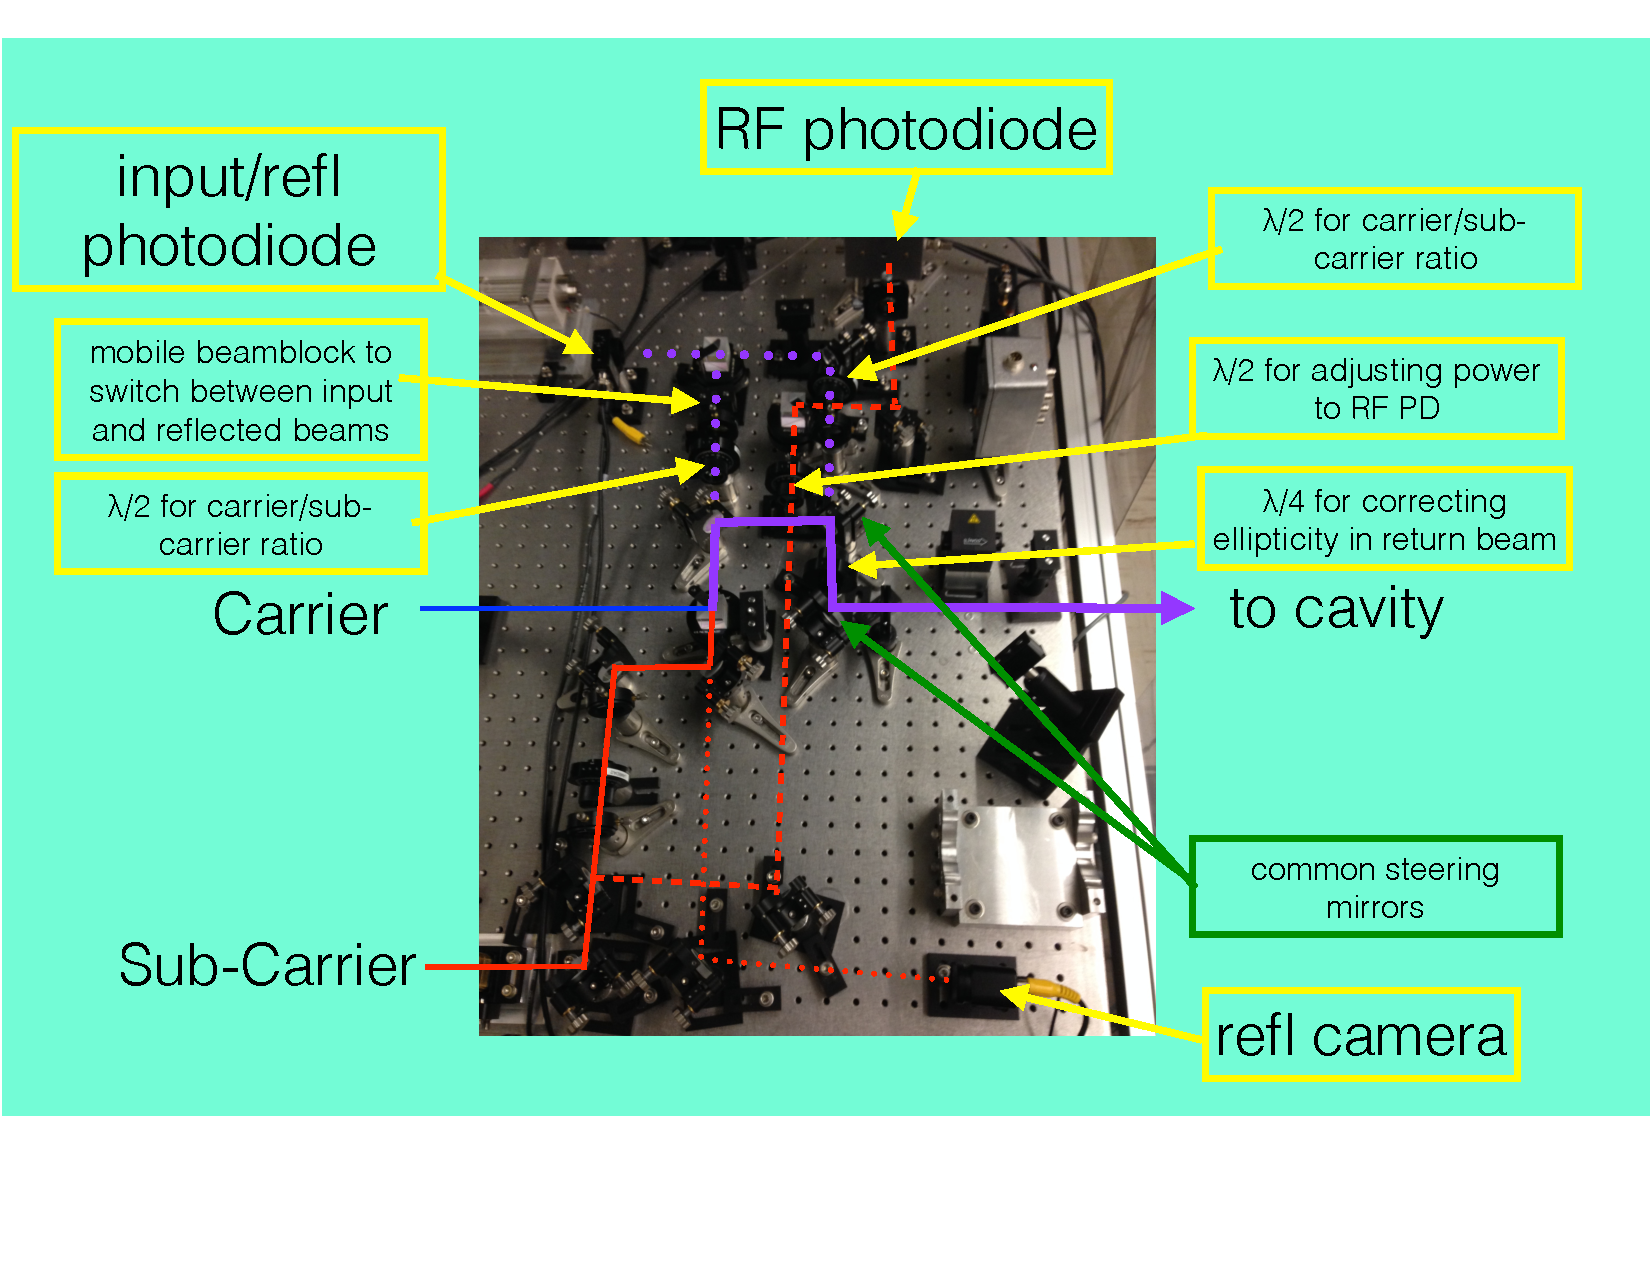
\includegraphics[width=15cm]{./figures/newinput.pdf}
  \caption[Table 1 Input Optics]{Table 1 Input Optics}
  \label{fig:newinput}
\end{figure}

\subsection{Faraday Isolator}
The Faraday isolator is composed of a Faraday rotator and two \ac{pbs} cubes.
The Faraday rotator is a medium which in the presence of a magnetic field
will rotate the polarization of light as it propagates through the medium.
There are other, much simpler devices that can rotate the polarization.
However, the advantage of the \ac{fi} is that it will rotate the polarization
in a fixed direction relative to the lab and not relative to the direction
of propagation.

In the case of the Faraday isolator, the polarization is rotated by 45 degrees
so that any reflected light comes back through the \ac{fi} with a 90 degree
rotation.
The isolation is then done by adding a \ac{pbs} cube at the input to the
Faraday rotator. Then we also add one on the output because there will often be
additional optics that will disturb the polarization of the reflected light
entering the \ac{fi} from the output side.
Another way of putting it is that the \ac{pbs} on the input side transmits
only the linear polarization that will transmit through the output \ac{pbs}.
The output \ac{pbs} transmits only the linear polarization that will be
reflected by the input \ac{pbs}.


\section{Linear Trap Experiment, 2nd Edition}
\label{sec:results_second}
With the changes described above in place, we were able to observe several
stable and unstable springs as before.
This time the measurement procedure was to vary the frequency offset between
carrier and subcarrier for each measurement, keeping the other settings fixed.
%We chose this procedure to eliminate any changes to the input power ratio
%caused by changing the subcarrier detuning. The subcarrier detuning changes the
%DC position of the input mirror by pushing on the mirror with our \ac{sos}
%\ac{osem}s. There is an angular coupling between the 
We chose this procedure to simplify the data fitting afterwards.
We know the subcarrier servo offset frequency with much better accuracy than we
know the subcarrier detuning.
Also, changing the subcarrier detuning changes the gain of the system to some
extent because the \ac{pdh} error signal is not linear at the scale of large
detuning changes. The change in gain due to subcarrier offset can be seen in
figure \ref{fig:aprilolg2}

\begin{figure}
\centering
  \tikzsetnextfilename{servoactuation}
  \begin{tikzpicture}
  \begin{loglogaxis}[
    name=plot1,
    height=6cm,
    ylabel={Magnitude},
    xlabel={Frequency [Hz]},
%    ylabel={Magnitude [dB]},
%    ymin=0,
%    xmin=32000000,
%    xmax=38000000,
    ymin=0.1,
    xmin=10,
    xmax=100000,
    grid=both,
  ]
    \addplot[red,very thick] table[x index=0,y index=1]
      {./matlab_traces/servoactuation.dat};
    \addlegendentry{OSEM};
    \addplot[blue,very thick] table[x index=0,y index=2]
      {./matlab_traces/servoactuation.dat};
    \addlegendentry{Laser PZT};
  \end{loglogaxis}
%  \begin{semilogxaxis}[
%    name=plot2,
%    at=(plot1.below south), anchor=above north,
%    height=4cm,
%    ylabel={Phase [Deg]},
%    xlabel={Frequency [Hz]},
%    xmin=10,
%    xmax=100000,
%    grid=both,
%    ]
%    \addplot[red,very thick] table[x index=0,y index=3]
%      {./matlab_traces/servoactuation.dat};
%    \addplot[blue,very thick] table[x index=0,y index=4]
%      {./matlab_traces/servoactuation.dat};
%  \end{semilogxaxis}
  \end{tikzpicture}
  \caption[Active Feedback Control for 2nd Edition]{
    Active feedback used for the second edition of the experiment.
    This shows each of the two actuation paths used with the
    crossover point.
    }
  \label{fig:servoactuation}
\end{figure}


For active feedback we used two actuation paths, one to the laser \ac{pzt} and
one to the \ac{osem} actuators which provide a force to the input mass.
The electronic servo which is common to both paths had the 100 Hz integrator
engaged.
This integrator has a flat response above 100 Hz and provides a boost below
100 Hz for better seismic suppression.
The two paths have a crossover frequency of 200Hz as can be seen in figure
\ref{fig:servoactuation}.


With the orthogonal polarization of the beams, we were able to monitor the
transmitted power for each beam.
The optical spring has four parameters that can change during the
measurement: carrier power, subcarrier power, carrier detuning, and subcarrier
detuning. The measurements of the carrier and subcarrier transmitted powers,
the observed resonant frequency, and the subcarrier servo offset form a set
of parameters from which we can determine the optical spring parameters leaving
us with no free parameters in the fitting.

Measurement parameters and spring frequencies can be seen in table
\ref{tab:experiment2params}.
The subcarrier detuning was set by checking the carrier power; then increasing
the subcarrier servo offset by 50kHz, which increases the carrier detuning by
50kHz because of the lock offset;
then changing the electronic offset for the subcarrier detuning to get back to
the original carrier transmitted power.
This procedure allowed us to use the well defined frequency offset from the
subcarrier servo to set the subcarrier detuning to -50kHz. The uncertainty
with this comes from noise in the transmitted carrier \ac{pd} signal relative
to the slope of W/Hz (Transmitted Power/Carrier Detuning).



\begin{table}
  \begin{center}
    \small
    \begin{tabular}{|l|l|l|}
      \hline
      Measurement ID & Subcarrier Servo Offset $[\mathrm{kHz}]$ & Resonant Frequency [Hz] \\
      \hline
      \hline
      2-13 & 330  & 274.8 \\
      2-20 & 330  & 370.7 \\
      2-10 & 320  & 424 \\
      2-15 & 300  & 609 \\
      2-18 & 260  & 915 \\
      2-19 & 240  & 1047 \\
      \hline
    \end{tabular}
  \end{center}
  \caption[Optical Trap, 2nd Edition Spring Measurements]{
      Parameters of measurements presented in figure \ref{fig:juneOLGresults}.
      }
  \label{tab:experiment2params}
\end{table}

When fitting the data using the technique above, we were not able to get the
stability to fit correctly, see figure \ref{fig:juneOLGresults_noabs}.
The measured springs were consistently more unstable than the model.
This gave an indication that our model must be missing some physics.
%The stability of the optical springs would not match with the theory without
%the addition of some extra physics.
With the addition of an effect from the thermal expansion of the high
reflective optical coatings, we were able to fit the stablility
properly.

%Thermal expansion couples in to the transfer function by the fact that driving
%the position of the mirror causes an intracavity power fluctuation and thus a
%temperature fluctuation in the surface of the mirror due to absorption.
%This temperature fluctuation causes a fluctuation in the thickness
%of the optic.
Thermal expansion couples into the transfer function by absorption of the
circulating power in the cavity at the surface of the mirror expanding the
optic and making the cavity length shorter.
This will be expained in more detail in section
\ref{sec:opticthermalexpansion}.
It turns out that only about 5ppm absorption is required to account for the
discrepancy in stablility.
This is, in part, due to the high circulating power and the small
beam spot size on the cavity end mirrors.
The results of this fitting can be seen in figure \ref{fig:juneOLGresults}.

\subsection{Optical Spring Cavity Residual Motion}

We want to know the residual motion of the cavity if we were to remove the
active feedback.
In order to do this we need to measure the control signal while locked with
a stable spring.
The control signal is the output of the feedback servo before the
actuation.
Since the error point (input to feedback servo) is set to zero by the
feedback servo below the unity gain frequency of the loop, the control
signal tells us what actuation is required to cancel noise entering the
system.
This allows us to estimate how much motion there would be if we remove
the active feedback loop.
Knowing the actuation transfer functions, we can convert the control signal
to the length noise entering the system.
%The sum of the two actuation paths and we'll call this $A$.
We have two actuation paths, to the laser and to the test mass actuator
(\ac{osem}) with a crossover frequency of 300Hz.
The sensing and feedback we will call $F$.
So the open loop gain is $AF$ in the absence of the optical spring.
With the optical spring, this becomes $\frac{AF}{1-O}$, where $O$ is the
open loop gain of the optical spring.
Closing the loop, the control signal $f$ will be,
\begin{align}
\frac{Fn}{1-\left(O+AF\right)} \label{eq:control} \;.
\end{align}
Since $AF$ is much larger than everything else in the denominator below
the unity gain frequency, we get,
\begin{equation}
f\approx -\frac{1}{A}n \label{eq:noisefunc} \;,
\end{equation}
where $n$ is the noise entering the system.
Taking the inverse of the equation \eqref{eq:control} gives us a function
to convert the measured control signal to the length noise entering the system.
We can then apply the closed loop gain of the optical spring loop to compute
what the residual length motion of the cavity would be in the absence of the
active feedback.
\begin{equation}
\frac{\left(1-O-AF\right)}{F\left(1-O\right)}f
\end{equation}
Since we have made a measurement $G$ that includes the optical spring,
\begin{equation}
G=\frac{AF}{1-O},
\end{equation}
We can replace $1-O$ in equation \eqref{eq:noisefunc} with
$\frac{AF}{G}$. With a bit of algrabra we get,
\begin{equation}
n = \frac{1-G}{F}f \;.
\end{equation}
The result of this measurement is shown in figure \ref{fig:noisepassive}
where the noise measurement was taken with the spring from measurement \#2-13.


It can be seen from the plot that the residual \ac{rms} motion is about
$1.3\times 10^{-11} \mathrm{m}$.
We want this to be less than the stability range as defined in
section \ref{sec:results_stability}.
%I say significantly because across the stability range the system is
%non-linear since the quality factor $Q$ of the spring increases toward
%edge of the range.
The response is non-linear for motion on the order of the stability range.


The stability range can be seen for various detunings in figure
\ref{fig:experiment2space}.
There is a trade off between phase and frequency however.
The lower phase will create a higher $Q$ spring resonance which will amplify the
noise entering the system at the resonance more than the higher phase/
lower $Q$ spring resonance.
At higher frequencies, the noise entering the system is enough lower to
compensate for the higher $Q$ (see fig. \ref{fig:rmsspringcompare})
so that we can reduce the overall rms motion.
We can also see that noise dominating the \ac{rms} motion at low frequencies
is from the bounce mode of our vertical isolation at about 7 Hz and
pure seismic takes over below about 3 Hz.

\subsubsection{Purely Passive Spring}
\label{sec:results2imp}

With a 800Hz optical spring using the same total input power used in this
experiment we see that we can get the \ac{rms} motion at
the resonance down to about the 2.5 pm limit.
This is marginally good enough at the resonance but we would still need active
feedback for the noise below 10Hz.

To improve the stability of the spring we have three main areas we can address:
the residual motion at the resonance frequency, the residual motion below 10
Hz, and the stability range itself.

At the resonant frequency we can
increase the laser power which we can use to increase the
spring frequency further, decrease the $Q$, or a combination
of the two.
The increased laser power will result in an increase in the intensity
noise however the limiting factor is still the laser frequency noise.

We can also decrease the noise entering the system at 800Hz. The limit here
is laser frequency noise.
We will need to implement the \ac{fss} in order to improve this, however
we need the full actuation range of the laser \ac{pzt} for lock acquisition.
Once lock is acquired
we can separately acquire the FSS and change the feedback scheme to make the
laser follow the reference cavity.
%we are basically using the feedback servo to stabilize
%the laser frequency, so we should be able to run the \ac{fss} open and tune
%the laser temperature to get the \ac{fss} error point aligned with the
%reference cavity.
This would drop the frequency noise down to the level of the \ac{vco} noise
which is at $0.1\mathrm{Hz/\sqrt{Hz}}$ at 800Hz, corresponding to
$2.5\times 10^{-17}\mathrm{Hz/\sqrt{Hz}}$.
Thus the noise budget would then be limited by the laser intensity noise, which
is at the level of about $5\times 10^{-16}\mathrm{Hz/\sqrt{Hz}}$ at 800 Hz.
%We can then do a control handoff for the frequency stabilization from the
%trap servo to the \ac{fss}.
This drops the overall noise at 800 Hz by a factor of 20, reducing the \ac{rms}
noise to roughly $1.3\times 10^{-13} \mathrm{m/\sqrt{Hz}}$.

For the low frequency motion we can simply keep the feedback engaged below 10Hz.
Also, by increasing laser power to improve the \ac{rms} motion at high
frequency, we
will also improve the \ac{rms} motion at low frequency, either by having a
stronger spring which will improve the low frequency suppression or by
increasing the phase of the optical spring which will increase the stability
range for the system.
Another option for improving the motion at low frequencies would be to add an
additional seismic isolation stage.
This would be a common isolation platform with a resonant frequency below
about 0.5 Hz.
The design is already partially complete on this, but was delayed due to
complexity.
The main difficulty with this will be controlling it below the resonant
frequency for alignment.





%So, this noise entering the system below the unity gain frequency will be
%$Af$, where $f$ is the control signal.


\subsection{Optic Thermal Expansion Contribution}
\label{sec:opticthermalexpansion}
The power fluctuations which provide the force feedback for the optical spring
also cause fluctuations of the absorbed power at the surface of the mirror.
This leads to thermal expension fluctuations of the mirror changing the length
of the cavity.
The effect was observed during initial LIGO as a noise coupling, see
\cite{Ballmer:thesis}.
The relevant part that we are interested in is the effect of changing
the thickness of the optic itself due to thermal expansion.

At the frequencies we're interested in, the depth of the thermal expansion
oscillations is very shallow compared to the thickness of the optic due to
the slow heat conduction through the optic substrate.
We want to first consider this penetration depth $d$ of the thermal
fluctuations. This is given by,
\begin{align}
\label{eq:pendepth}
d &= \sqrt{\frac{\kappa}{2\pi fC\rho}} = 18.4 \mathrm{\mu m}
     \sqrt{\frac{400 \mathrm{Hz}}{f}} \,.
\end{align}
I have written the equation in this form to illustrate that at the lower
optical spring frequencies from the experiment, we have a maximum penetration
depth of about $18\mathrm{\mu m}$.
This is nearly an order of magnitude smaller than the beam spot diameter, which
is about $320\mu m$. The change in thickness $\Delta z$ of the optic can then
be approximated with
\begin{equation} \label{eq:deltaz}
\Delta z = \left(1+\eta\right)\alpha\frac{ \delta P }{2\pi ifC\rho A} \, ,
\end{equation}
where $\delta$ is the absorption coefficient, $A$ is the area of the beam,
$\alpha$ is the linear coefficient of thermal expansion, and $\eta$ is the
Poisson ratio.

From equation \ref{eq:deltaz} we can get the transfer function from force to
traplength. With a factor of $c/2$ to remove the optical power to force from
the optical spring $K_{OS}$, the transfer function depicted in figure
\ref{fig:traploopCTE} is
\begin{equation}
\frac{-c \delta \alpha \left(1+\eta\right)}{4\pi ifC\rho A} \, .
\end{equation}

The majority of the change in power buildup due to cavity length is due to the
carrier beam which has a positive detuning.
Because of this detuning, expansion of the optics will shorten the cavity and
increase the intracavity power.
The intracavity power fluctuations will thus have a positive feedback and add
to the instability of the optical spring.

\begin{figure}
\centering
\tikzsetnextfilename{traploopCTE}
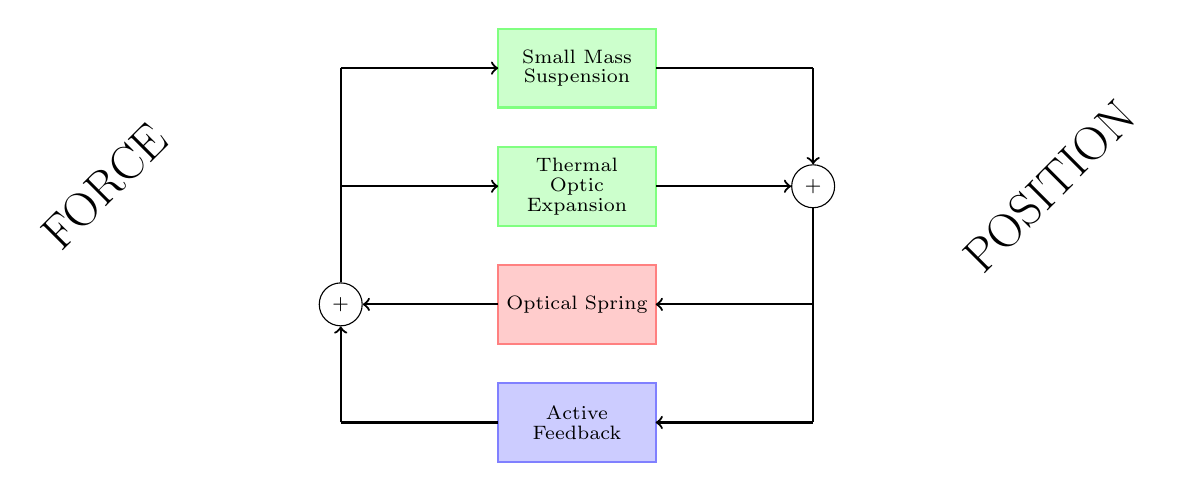
\begin{tikzpicture}[
  analog/.style={rectangle,draw=blue!50,fill=blue!20,thick,align=center,
    outer sep=0,minimum width=2cm,
    minimum height=1cm,
    text width=1.8cm},
  digital/.style={rectangle,draw=black!50,fill=black!20,thick,align=center,
    outer sep=0,minimum width=2cm,
     minimum height=1cm,
    text width=1.8cm},
  physical/.style={rectangle,draw=green!50,fill=green!20,thick,align=center,
    outer sep=0,minimum width=2cm,
    minimum height=1cm,
    text width=1.8cm},
  optical/.style={rectangle,draw=red!50,fill=red!20,thick,align=center,
    outer sep=0,minimum width=2cm,
    minimum height=1cm,
    text width=1.8cm}]
  \renewcommand{\baselinestretch}{0.9}
  \begin{scriptsize}
  \node[circle,draw=black] (sum1) at (-3,-1.5) {$+$};
  \node[circle,draw=black] (sum2) at (3,0) {$+$};
  \node[analog] (F) at (0,-3) {Active Feedback};
  \node[optical] (O) at (0,-1.5) {Optical Spring};
  \node[physical] (S) at (0,1.5) {Small Mass Suspension};
  \node[physical] (CTE) at (0,0) {Thermal Optic Expansion};
  \coordinate (j1) at (-3,-3) {};
  \coordinate (j2) at (-3,-1.5) {};
  \coordinate (j3) at (-3,0) {};
  \coordinate (j4) at (-3,1.5) {};
  \coordinate (j5) at (3,-3) {};
  \coordinate (j6) at (3,-1.5) {};
  \coordinate (j7) at (3,0) {};
  \coordinate (j8) at (3,1.5) {};
  \draw[thick] (F) -- (j1);
  \draw[thick,->] (O) -- (sum1);
  \draw[thick,->] (j3) -- (CTE);
  \draw[thick,->] (j4) -- (S);
  \draw[thick,->] (j1) -- (sum1);
  \draw[thick] (sum1) -- (j3);
  \draw[thick] (j3) -- (j4);
  \draw[thick,<-] (F) -- (j5);
  \draw[thick,<-] (O) -- (j6);
  \draw[thick,<-] (sum2) -- (CTE);
  \draw[thick] (j8) -- (S);
  \draw[thick] (j5) -- (j6);
  \draw[thick] (j6) -- (sum2);
  \draw[thick,<-] (sum2) -- (j8);
  \node[rotate=45] (force) at (-6,0) {\LARGE FORCE};
  \node[rotate=45] (pos) at (6,0) {\LARGE POSITION};
  \end{scriptsize}
\end{tikzpicture}
  \caption[Trap Loop With Optic Thermal Expansion]{
    This shows how the thermal expansion effect couples into the experiment.
    Active feedback represents the two feedback paths displayed in figure
    \ref{fig:traploops}.
    }
  \label{fig:traploopCTE}
\end{figure}


\begin{figure}
  \tikzsetnextfilename{juneOLGresults}
  \begin{tikzpicture}
  \begin{loglogaxis}[
    name=plot1,
    height=7cm,
    width=14cm,
    xmin=100,
    xmax=2000,
    xtick={1e2,1e3},
    ylabel={Magnitude},
    grid=both,
  ]
  \addplot[blue,very thick,smooth,dashed] table[x index=0,y index=1]
    {./matlab_traces/juneResults13fit.dat};
  \addplot[green,very thick,smooth,dashed] table[x index=0,y index=1]
    {./matlab_traces/juneResults20fit.dat};
  \addplot[red,very thick,smooth,dashed] table[x index=0,y index=1]
    {./matlab_traces/juneResults10fit.dat};
  \addplot[teal,very thick,smooth,dashed] table[x index=0,y index=1]
    {./matlab_traces/juneResults15fit.dat};
  \addplot[magenta,very thick,smooth,dashed] table[x index=0,y index=1]
    {./matlab_traces/juneResults18fit.dat};
  \addplot[yellow,very thick,smooth,dashed] table[x index=0,y index=1]
    {./matlab_traces/juneResults19fit.dat};
  \addplot[blue,very thick,smooth] table[x index=0,y index=1] {./matlab_traces/juneResults13.dat};
  \addplot[green,very thick,smooth] table[x index=0,y index=1] {./matlab_traces/juneResults20.dat};
  \addplot[red,very thick,smooth] table[x index=0,y index=1] {./matlab_traces/juneResults10.dat};
  \addplot[teal,very thick,smooth] table[x index=0,y index=1] {./matlab_traces/juneResults15.dat};
  \addplot[magenta,very thick,smooth] table[x index=0,y index=1] {./matlab_traces/juneResults18.dat};
  \addplot[yellow,very thick,smooth] table[x index=0,y index=1] {./matlab_traces/juneResults19.dat};
  \end{loglogaxis}
  \begin{semilogxaxis}[
    name=plot2,
    at=(plot1.below south), anchor=above north,
    height=7cm,
    width=14cm,
    xmin=100,
    xmax=2000,
    xtick={1e2,1e3},
    xlabel={Frequency [Hz]},
    ylabel={Phase [Deg]},
    legend style={legend pos=north west,font=\tiny},
    grid=both,
  ]
  \addplot[blue,very thick,dashed,forget plot] table[x index=0,y index=2]
    {./matlab_traces/juneResults13fit.dat};
  \addplot[green,very thick,dashed,forget plot] table[x index=0,y index=2]
    {./matlab_traces/juneResults20fit.dat};
  \addplot[red,very thick,dashed,forget plot] table[x index=0,y index=2]
    {./matlab_traces/juneResults10fit.dat};
  \addplot[teal,very thick,dashed,forget plot] table[x index=0,y index=2]
    {./matlab_traces/juneResults15fit.dat};
  \addplot[magenta,very thick,dashed,forget plot] table[x index=0,y index=2]
    {./matlab_traces/juneResults18fit.dat};
  \addplot[yellow,very thick,dashed,forget plot] table[x index=0,y index=2]
    {./matlab_traces/juneResults19fit.dat};
  \addplot[blue,very thick] table[x index=0,y index=2] {./matlab_traces/juneResults13.dat};
  \addlegendentry{DetC=290.8kHz,DetS=-39.2kHz,Pratio=3.46}
  \addplot[green,very thick] table[x index=0,y index=2] {./matlab_traces/juneResults20.dat};
  \addlegendentry{DetC=285.0kHz,DetS=-45.0kHz,Pratio=3.96}
  \addplot[red,very thick] table[x index=0,y index=2] {./matlab_traces/juneResults10.dat};
  \addlegendentry{DetC=285.1kHz,DetS=-34.9kHz,Pratio=3.50}
  \addplot[teal,very thick] table[x index=0,y index=2] {./matlab_traces/juneResults15.dat};
  \addlegendentry{DetC=264.2kHz,DetS=-35.8kHz,Pratio=3.94}
  \addplot[magenta,very thick] table[x index=0,y index=2] {./matlab_traces/juneResults18.dat};
  \addlegendentry{DetC=238.2kHz,DetS=-21.8kHz,Pratio=4.27}
  \addplot[yellow,very thick] table[x index=0,y index=2] {./matlab_traces/juneResults19.dat};
  \addlegendentry{DetC=222.5kHz,DetS=-17.5kHz,Pratio=4.42}
  \end{semilogxaxis}
  \end{tikzpicture}
    \caption[Data Fitting of Open Loop Gain for 2nd Results]{This is the open
      loop gain fit for the second edition of the experiment.
      The solid lines are the measured
      optical spring transfer functions. The dashed lines are the corresponding
      theoretical transfer functions. In the legend, "DetC" and "DetS" stand for
      carrier and subcarrier detuning respectively. Pratio is the power ratio
      of carrier to subcarrier input power.}
  \label{fig:juneOLGresults}
\end{figure}

\begin{figure}
\centering
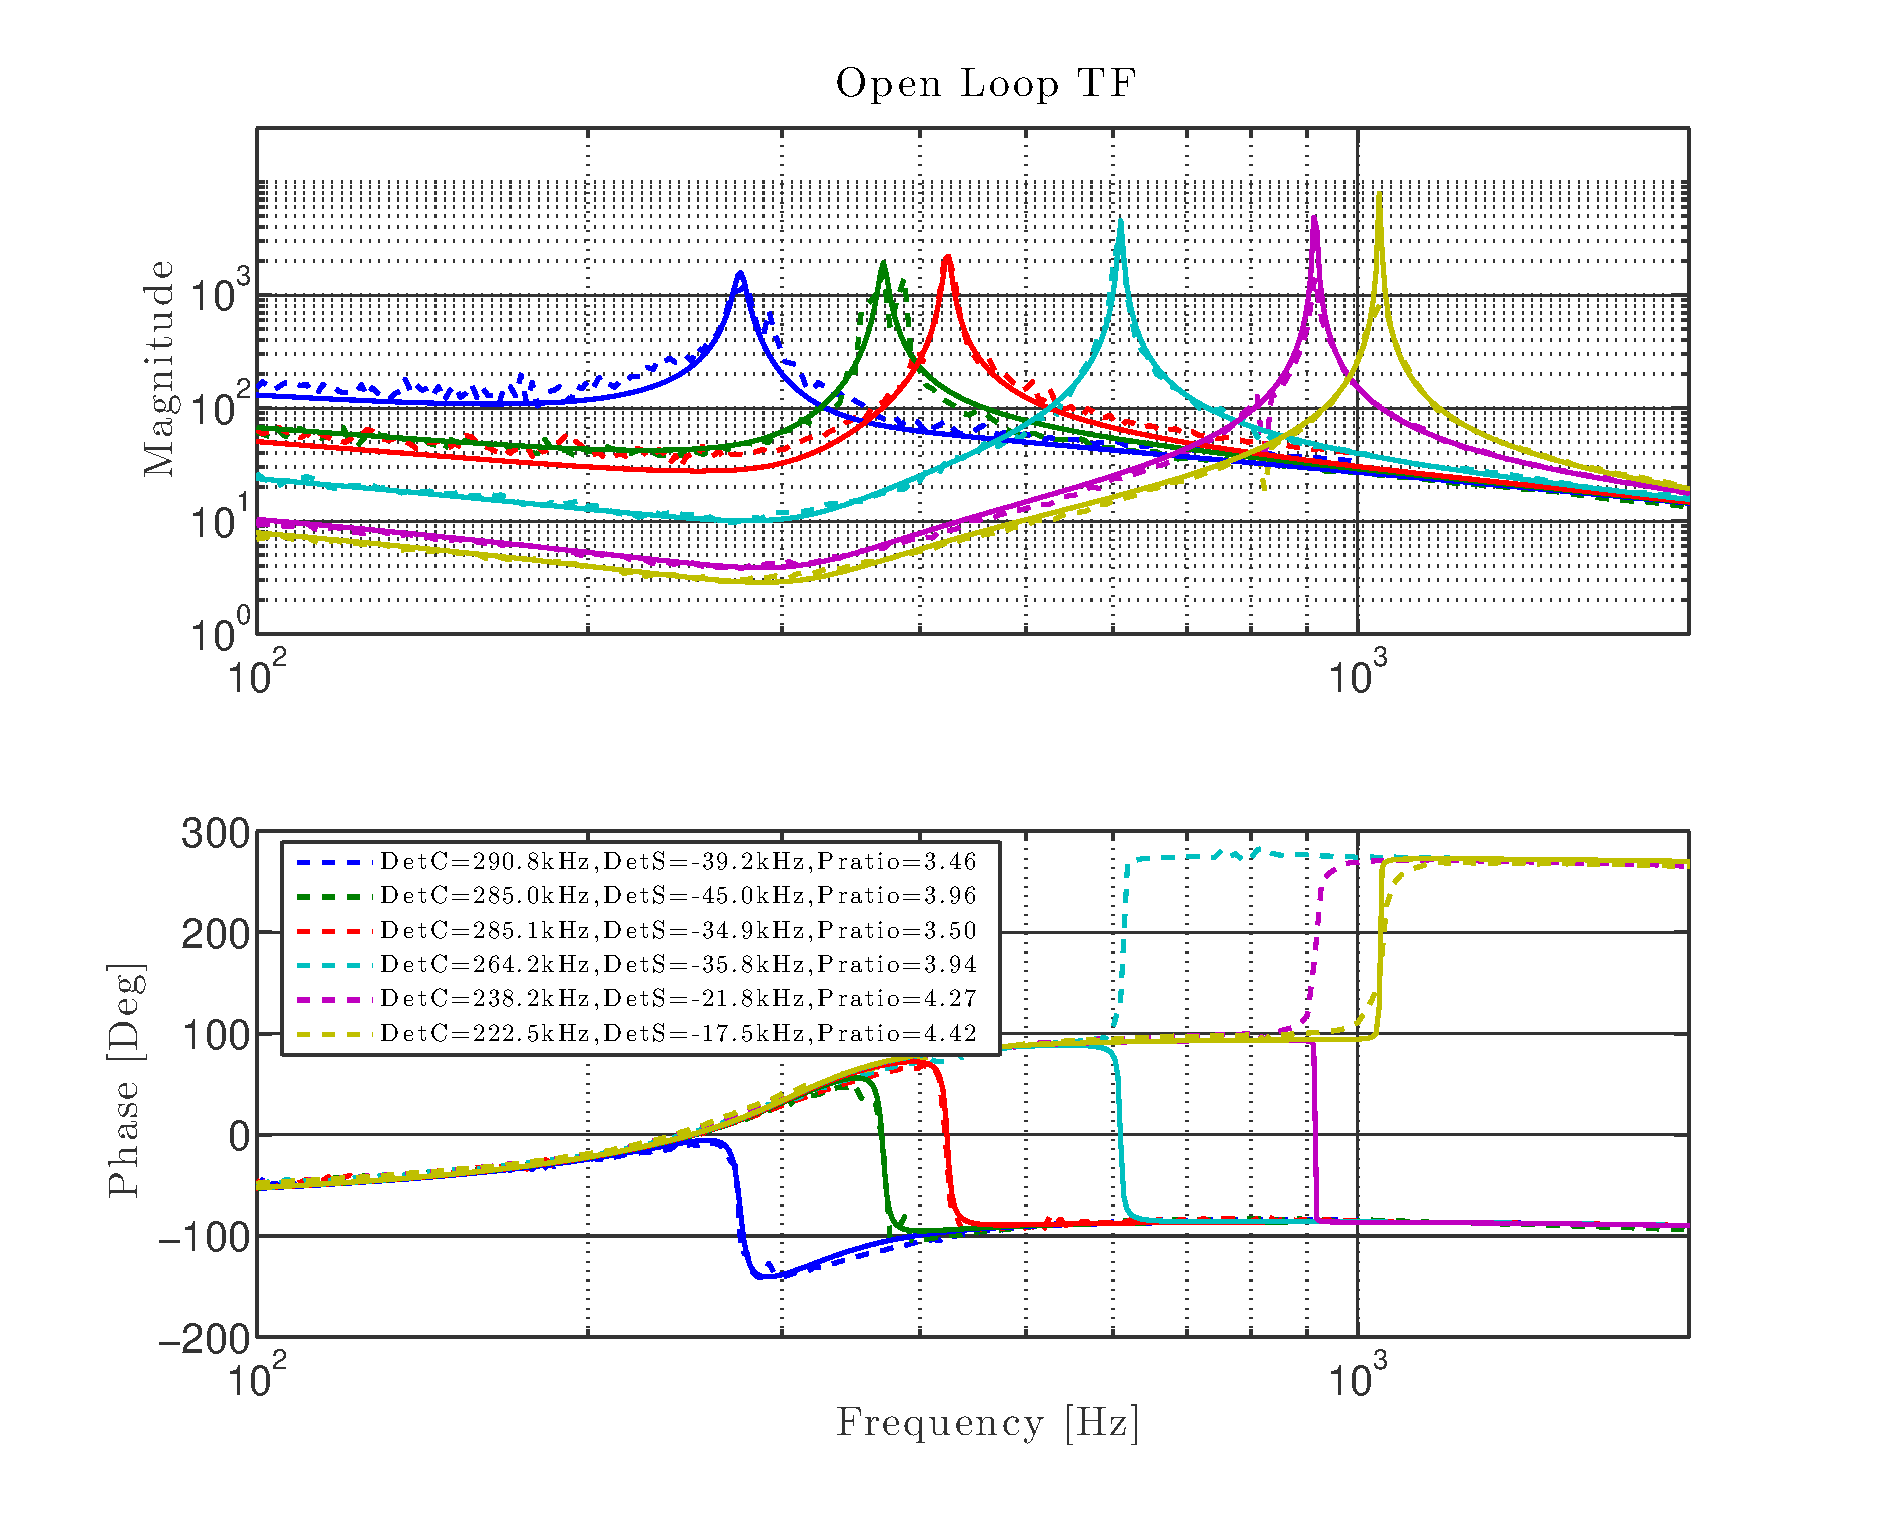
\includegraphics[width=14cm]{./figures/spring2noabs}
\caption[Data Fitting Without Absorption Coefficient]{
  Open loop gain measurements of the second edition of the experiment.
  This plot shows the fit without the absorption term.
  Two of the optical springs become stable which does not match with the
  measurement.
  }
\label{fig:juneOLGresults_noabs}
\end{figure}


\begin{table}
  \begin{center}
    \footnotesize
    \begin{tabular}{|l|l|l|l|l|}
      \hline
      Measurement & Carrier & Subcarrier & Carrier & Subcarrier \\
      ID & Detuning $[\mathrm{kHz}]$ & Detuning $[\mathrm{kHz}]$ &
        Power [mW] & Power [mW] \\
      \hline
      \hline
      2-13 & 290.8  & -39.2  & 215.9 & 62.5 \\
      2-20 & 285.0  & -45.0  & 213.3 & 53.8 \\
      2-10 & 285.1  & -34.9  & 223.0 & 63.7 \\
      2-15 & 264.2  & -35.8  & 215.2 & 54.6 \\
      2-18 & 238.2  & -21.8  & 224.2 & 52.5 \\
      2-19 & 222.5  & -17.5  & 228.5 & 51.7 \\
      \hline
    \end{tabular}
  \end{center}
  \caption[Optical Trap, 2nd Edition Optical Spring Fit Parametrers]{
      Parameters of measurements presented in figure \ref{fig:juneOLGresults}.
      }
  \label{tab:experiment2fitparams}
\end{table}

\begin{figure}
  \tikzsetnextfilename{noisepassive}
  \begin{tikzpicture}
  \begin{loglogaxis}[
    height=12cm,
    width=14cm,
    xlabel={Frequency $\left[\mathrm{Hz}\right]$},
    ylabel={Trap Length Noise $\left[\mathrm{m}/\sqrt{\mathrm{Hz}}\right]$},
    xmin=10,
    xmax=6000,
    ymin=1e-16,
    ymax=1e-8,
    grid=major,
    legend cell align=left,
  ]
  \addplot[blue,very thick,smooth] table[x index=0,y index=1]
    {./matlab_traces/june_noises.dat};
  \addlegendentry{Measured Trap Length Noise}
  \addplot[red,very thick,smooth] table[x index=0,y index=5]
    {./matlab_traces/june_noises.dat};
  \addlegendentry{Trap Length Noise Without Active Feedback}
  \addplot[red,dashed,very thick,smooth] table[x index=0,y index=6]
    {./matlab_traces/june_noises.dat};
  \addlegendentry{Trap Length RMS Without Active Feedback}
  \end{loglogaxis}
  \end{tikzpicture}
    \caption[Estimate of Passively Attenuated Noise]{
    This is the noise budget which includes the measured
    cavity length noise with a stable optical spring.
    }
  \label{fig:noisepassive}
\end{figure}


